% ============================================================================
% LSA-BASED STACKING ENSEMBLE WITH GRANULARITY ANALYSIS
% FOR EMOTION CLASSIFICATION ON INDONESIAN SOCIAL MEDIA
% A Complete Guide: From Business Problem to Publication-Ready Results
% ============================================================================
\documentclass[12pt,a4paper,twoside]{article}

% --- Packages ---
\usepackage[utf8]{inputenc}
\usepackage[T1]{fontenc}
\usepackage{lmodern}
\usepackage[margin=1in]{geometry}
\usepackage{amsmath,amssymb,amsthm,mathtools}
\usepackage{graphicx}
\usepackage{xcolor}
\usepackage{hyperref}
\usepackage{booktabs}
\usepackage{longtable}
\usepackage{enumitem}
\usepackage{tcolorbox}
\usepackage{fancyhdr}
\usepackage{titlesec}
\usepackage{caption}
\usepackage{subcaption}
\usepackage{algorithm}
\usepackage{algpseudocode}
\usepackage{natbib}
\usepackage{tocloft}
\usepackage{setspace}
\usepackage{tikz}
\usetikzlibrary{arrows.meta,positioning,shapes.geometric}
\usepackage{capt-of}
\usepackage{multirow}
\usepackage{array}
\graphicspath{{../outputs/figures/}}

% Simple watermark
\usepackage{draftwatermark}
\SetWatermarkText{HILMI}
\SetWatermarkScale{1.0}
\SetWatermarkColor[gray]{0.92}
\SetWatermarkAngle{0}

% --- Colors ---
\definecolor{mainblue}{RGB}{31,78,121}
\definecolor{accentorange}{RGB}{230,126,34}
\definecolor{notegray}{RGB}{245,245,245}
\definecolor{noteborder}{RGB}{180,180,180}
\definecolor{darktext}{RGB}{44,62,80}
\definecolor{lightblue}{RGB}{235,245,252}

% --- Hyperref setup ---
\hypersetup{
    colorlinks=true,
    linkcolor=mainblue,
    citecolor=mainblue,
    urlcolor=accentorange,
    bookmarksdepth=3
}

% --- Note box environment ---
\newtcolorbox{notebox}[1][]{
    colback=notegray,
    colframe=noteborder,
    fonttitle=\bfseries,
    title={#1},
    boxrule=0.5pt,
    arc=2pt,
    left=8pt,
    right=8pt,
    top=6pt,
    bottom=6pt
}

% --- File reference box ---
\newtcolorbox{filebox}{
    colback=lightblue,
    colframe=mainblue!50,
    boxrule=0.4pt,
    arc=2pt,
    left=8pt,
    right=8pt,
    top=4pt,
    bottom=4pt
}

% --- Headers/Footers ---
\pagestyle{fancy}
\fancyhf{}
\fancyhead[LE,RO]{\thepage}
\fancyhead[RE]{\textit{LSA Stacking Ensemble for Emotion Classification}}
\fancyhead[LO]{\textit{\nouppercase{\leftmark}}}
\renewcommand{\headrulewidth}{0.4pt}

% --- Section formatting ---
\titleformat{\section}
  {\color{mainblue}\Large\bfseries}{\thesection}{1em}{}
\titleformat{\subsection}
  {\color{mainblue}\large\bfseries}{\thesubsection}{1em}{}
\titleformat{\subsubsection}
  {\color{mainblue}\normalsize\bfseries}{\thesubsubsection}{1em}{}

% --- Theorem environments ---
\theoremstyle{definition}
\newtheorem{definition}{Definition}[section]

% --- Spacing ---
\setlength{\parskip}{6pt}
\setlength{\parindent}{0pt}

% ============================================================================
% DOCUMENT BEGIN
% ============================================================================
% SET YOUR FIGURE PATH HERE:
% \graphicspath{{D:/Research (Read every day!)/Project Data/mentoring/multitopic_project/outputs/figures/}}
\begin{document}

% ============================================================================
% TITLE PAGE
% ============================================================================
\begin{titlepage}
\centering
\vspace*{2cm}

{\color{mainblue}\rule{\textwidth}{2pt}}
\vspace{0.5cm}

{\Huge\bfseries\color{mainblue} Decoding Emotions in the\\Comment Section\\[0.3cm]}
{\LARGE\color{darktext} LSA Stacking Ensemble with Granularity Analysis\\for Emotion Classification on Indonesian Social Media}

\vspace{0.5cm}
{\color{mainblue}\rule{\textwidth}{2pt}}

\vspace{1.5cm}

{\Large By Hilmi}

\vspace{2cm}

\begin{flushleft}
\small
\textbf{Research Areas:} Natural Language Processing $\cdot$ Text Mining $\cdot$ Emotion Detection\\[0.3cm]
\textbf{Key Methods:} Latent Semantic Analysis $\cdot$ Stacking Ensemble $\cdot$ SMOTE $\cdot$ TF\,--\,IDF\\[0.3cm]
\textbf{Application Domain:} Indonesian Social Media $\cdot$ Javanese Dialect $\cdot$ Instagram Comments
\end{flushleft}

\vfill

\end{titlepage}

% ============================================================================
% PROJECT STATEMENT (1 page, before TOC)
% ============================================================================
\newpage
\thispagestyle{empty}

\begin{center}
{\Large\bfseries\color{mainblue} Project Statement}
\end{center}

\vspace{0.5cm}

My work sits at the intersection of \textbf{natural language processing}, \textbf{machine learning}, and \textbf{Indonesian digital culture}. I am motivated by a practical question: \textit{Can we build systems that reliably understand how Indonesian people feel when they express themselves online, even when they write in regional dialects and informal language?}

\textbf{Emotion analysis} is the foundation of understanding public sentiment, brand perception, and community well\,being on social media. While the field has matured significantly for English text, Indonesian language processing faces unique challenges. Indonesia has over 700 regional languages, and social media users frequently mix formal Indonesian (Bahasa Indonesia) with Javanese, Sundanese, or other local dialects. A comment like \textit{``Josss tenan''} (Javanese for ``Really awesome'') carries clear emotional content, but most existing NLP models trained on formal Indonesian would struggle with it.

\textbf{Why this project matters.} This research tackles the emotion classification problem specifically on Instagram comments from a regional television broadcaster (JTV Surabaya), where users write in a rich mixture of Indonesian and Javanese. The dataset is inherently challenging: it is highly imbalanced (73\% neutral), contains very short texts (median 3 words), and uses non\,standard spelling and slang. These are exactly the conditions where standard approaches fail.

\textbf{The technical contribution.} This project provides a systematic investigation of how \textbf{Latent Semantic Analysis (LSA)} topic dimensionality affects emotion classification quality when combined with a \textbf{stacking ensemble} of Random Forest, SVM, and XGBoost classifiers. Rather than choosing an arbitrary number of LSA topics, I test five granularities (k$=$5, 10, 25, 50, 100) and discover that \textbf{k$=$25 is optimal} for this type of short social media text. I also investigate whether combining multiple topic granularities simultaneously could improve results, and provide a carefully documented negative finding that is itself valuable for the community.

\textbf{What I learned.} The most important lesson came from failure. My initial 5\,class classifier achieved 0.00 F1\,score on two emotion classes (fear and sadness), which meant the model was predicting ``neutral'' for almost everything. Rather than reporting inflated accuracy, I diagnosed the problem (insufficient minority class samples), applied a principled class consolidation strategy, rebuilt the entire pipeline, and produced results where every class is meaningfully classified. This experience reinforced that \textbf{honest evaluation matters more than impressive numbers}.

I see this project as part of a broader effort to make NLP work for underrepresented languages and dialects, ensuring that communities like East Java's social media users are not left behind by the global advancement of language technology.

% ============================================================================
% TABLE OF CONTENTS
% ============================================================================
\newpage
\tableofcontents
\newpage

% ============================================================================
% SECTION 1: THE BUSINESS PROBLEM
% ============================================================================
\section{The Business Problem: Why Emotion Classification Matters}
\label{sec:business}

\subsection{Understanding the Audience}

Imagine you are the social media manager for a regional television broadcaster in East Java, Indonesia. Every day, thousands of viewers leave comments on your Instagram posts, reacting to shows, news segments, events, and promotions. These comments contain a wealth of information about how your audience feels, what they enjoy, what frustrates them, and what they want more of.

The challenge is that reading through thousands of comments manually is impractical. You need an automated system that can classify each comment into an emotion category, allowing you to answer questions like:

\begin{enumerate}[leftmargin=2em]
    \item Which programs generate the most positive emotional response?
    \item Are there topics that consistently trigger negative reactions?
    \item How does audience sentiment change around specific events?
    \item Which types of content should we produce more (or less) of?
\end{enumerate}

This is the \textbf{emotion classification problem}: given a short text comment, automatically determine the emotion it expresses.

\subsection{Why This Is Harder Than It Looks}

Several factors make emotion classification on Indonesian social media particularly challenging:

\begin{enumerate}[leftmargin=2em]
    \item \textbf{Regional dialect mixing.} Comments like ``Wuiiiiih segerrrr rek'' mix informal Indonesian with Javanese (``rek'' is a Surabayan address term). Standard Indonesian NLP tools often mishandle these tokens.

    \item \textbf{Extreme brevity.} The median comment length is only 3 words. With so little context, even humans sometimes disagree on the emotion.

    \item \textbf{Severe class imbalance.} Neutral comments vastly outnumber emotional ones (73\% neutral vs.\ 1\% fear). A naive classifier that always predicts ``neutral'' achieves 73\% accuracy, which sounds good but is useless.

    \item \textbf{Ambiguous emotions.} Comments like ``Waduh.. teganya'' (``Wow.. how heartless'') could express anger, sadness, or even humor depending on context.
\end{enumerate}

\begin{notebox}[The Business Objective]
Build a classification system that can reliably categorize Instagram comments into emotion classes, with particular attention to correctly identifying emotional (non\,neutral) comments. The system should work with short, informal, dialect\,heavy Indonesian text and handle severe class imbalance gracefully.
\end{notebox}

\subsection{From Business Problem to Technical Approach}

The business problem translates into the following technical pipeline:

\begin{enumerate}[leftmargin=2em]
    \item \textbf{Data collection and labeling:} Gather Instagram comments and assign emotion labels.
    \item \textbf{Text preprocessing:} Clean, normalize, tokenize, and stem the text.
    \item \textbf{Feature extraction:} Convert text into numerical features using TF\,--\,IDF and LSA.
    \item \textbf{Class imbalance handling:} Apply SMOTE to address the minority class problem.
    \item \textbf{Model training and evaluation:} Train classifiers and evaluate using metrics appropriate for imbalanced data.
\end{enumerate}

Each of these steps is implemented in the project code and explained in detail throughout this document.


\subsection{Real World Business Applications}
 
To make the value of emotion classification concrete, consider these specific scenarios where a broadcaster like JTV Surabaya could use the system built in this project.
 
\textbf{Content Strategy Optimization.} By classifying emotions on comments across different show types (news, entertainment, cultural programs), the social media team can identify which content formats generate the most positive engagement. If entertainment posts consistently receive ``joy'' responses while news posts receive more ``negative'' responses, the programming team can adjust the tone, format, or scheduling of different content types.
 
\textbf{Crisis Detection and Response.} A sudden spike in ``negative'' comments on a specific post may indicate a public relations issue, a controversial segment, or a technical broadcast problem. Real time emotion classification allows the social media team to detect and respond to these situations within minutes rather than hours.
 
\textbf{Audience Segmentation.} By analyzing emotion patterns per user over time, the marketing team can segment the audience into groups: enthusiastic supporters (frequent ``joy''), constructive critics (occasional ``negative'' with specific feedback), and passive viewers (mostly ``neutral''). Each segment can receive tailored engagement strategies.
 
\textbf{Advertiser Insights.} Advertisers want to place their products alongside positive content. Emotion classification enables JTV to provide advertisers with data showing which time slots and programs generate the most positive audience sentiment, justifying premium advertising rates.
 
\textbf{Competitor Benchmarking.} The same classification system can be applied to competitor Instagram accounts, allowing JTV to compare audience sentiment across regional broadcasters and identify competitive advantages.
 
\begin{notebox}[From Classification to Action]
The value of emotion classification is not in the classification itself, but in the \textbf{decisions} it enables. A broadcaster that knows 60\% of comments on their new show are ``joy'' and 15\% are ``negative'' can make informed programming decisions. Without classification, they have 3{,}700 unstructured comments and no actionable insight.
\end{notebox}


% ============================================================================
% SECTION 2: THE DATASET
% ============================================================================
\section{The Dataset: Instagram Comments from JTV Surabaya}
\label{sec:dataset}

\subsection{Data Source and Collection}

The dataset consists of 3{,}704 Instagram comments collected from the official account of JTV (Jawa Timur Television), a regional television broadcaster based in Surabaya, East Java, Indonesia (\texttt{@jtv\_rek}). JTV serves as a cultural hub for the East Java community, broadcasting local news, entertainment, and cultural programs in both Indonesian and Javanese.

The comments span a variety of post types: entertainment show reactions, news segment responses, event announcements, promotional content, and community engagement posts. Collection covered the period from January to April 2025.

\subsection{Annotation Scheme}

Each comment was annotated with one of five emotion labels following the basic emotion framework commonly used in Indonesian NLP research \citep{saputri2018emotion}:

\begin{enumerate}[leftmargin=2em]
    \item \textbf{Joy:} Comments expressing happiness, excitement, appreciation, or positive affect. Example: ``Seru banget'' (``So fun'').
    \item \textbf{Anger:} Comments expressing frustration, outrage, or dissatisfaction. Example: ``Memperburuk citra penyelenggara'' (``Worsening the organizer's image'').
    \item \textbf{Sadness:} Comments expressing sorrow, disappointment, or loss. Example: ``Acaranya sudah tidak ada lagi ya'' (``The show is no longer on, huh'').
    \item \textbf{Fear:} Comments expressing worry, anxiety, or concern. Example: ``Akun stasiun dangdut ilang ta?'' (``Did the dangdut station account disappear?'').
    \item \textbf{Neutral:} Comments that are informational, questions, or carry no strong emotion. Example: ``Syarat ketentuan min'' (``Terms and conditions, admin'').
\end{enumerate}

\subsection{Dataset Statistics}

After cleaning (removing 2 rows with missing text and 2 with missing labels), the final dataset contains 3{,}700 labeled comments.

\begin{table}[h]
\centering
\caption{Original 5\,class emotion distribution.}
\label{tab:dist5}
\begin{tabular}{lrr}
\toprule
\textbf{Emotion} & \textbf{Count} & \textbf{Percentage} \\
\midrule
Neutral & 2{,}704 & 73.1\% \\
Joy & 637 & 17.2\% \\
Anger & 235 & 6.4\% \\
Sadness & 84 & 2.3\% \\
Fear & 40 & 1.1\% \\
\midrule
\textbf{Total} & \textbf{3{,}700} & \textbf{100\%} \\
\bottomrule
\end{tabular}
\end{table}

The imbalance ratio (majority to minority class) is \textbf{67.6:1}, which is extreme. The fear class has only 40 samples total, meaning only approximately 8 samples would appear in a 20\% test set.

\begin{filebox}
\textbf{Code Reference:} The exploratory data analysis is performed in \texttt{step1\_eda\_preprocessing.py}. This script generates three figures: \texttt{fig1\_label\_distribution.png} (bar and pie chart of emotion distribution), \texttt{fig2\_text\_length\_analysis.png} (histogram and box plot of text lengths per emotion), and \texttt{fig3\_word\_frequency\_per\_emotion.png} (top 15 words for each emotion class).
\end{filebox}

\subsection{Text Characteristics}

The comments exhibit several notable characteristics:

\begin{enumerate}[leftmargin=2em]
    \item \textbf{Very short texts.} The average text length is 5.15 words, with a median of 3 words. Many comments are single words or short phrases (``Mantap'', ``Keren'', ``Josss tenan'').

    \item \textbf{Dialect mixing.} Comments frequently use Javanese terms: ``rek'' (form of address), ``lur'' (brother/friend), ``nang'' (at/to), ``isok'' (can), and ``wes'' (already).

    \item \textbf{Elongated words.} Users express emphasis through repetition: ``seruuuu'', ``mantaaaaaab'', ``wenaaakkk''.

    \item \textbf{Emotion words differ by class.} Anger comments tend to be longer (mean 8.45 words) and contain words like ``teganya'' (heartless), ``buruk'' (bad), ``paksa'' (force). Joy comments are shorter (mean 4.02 words) and contain words like ``seru'' (fun), ``keren'' (cool), ``mantap'' (great).
\end{enumerate}

% --- INSERT FIGURE HERE ---
% \begin{figure}[h]
% \centering
% 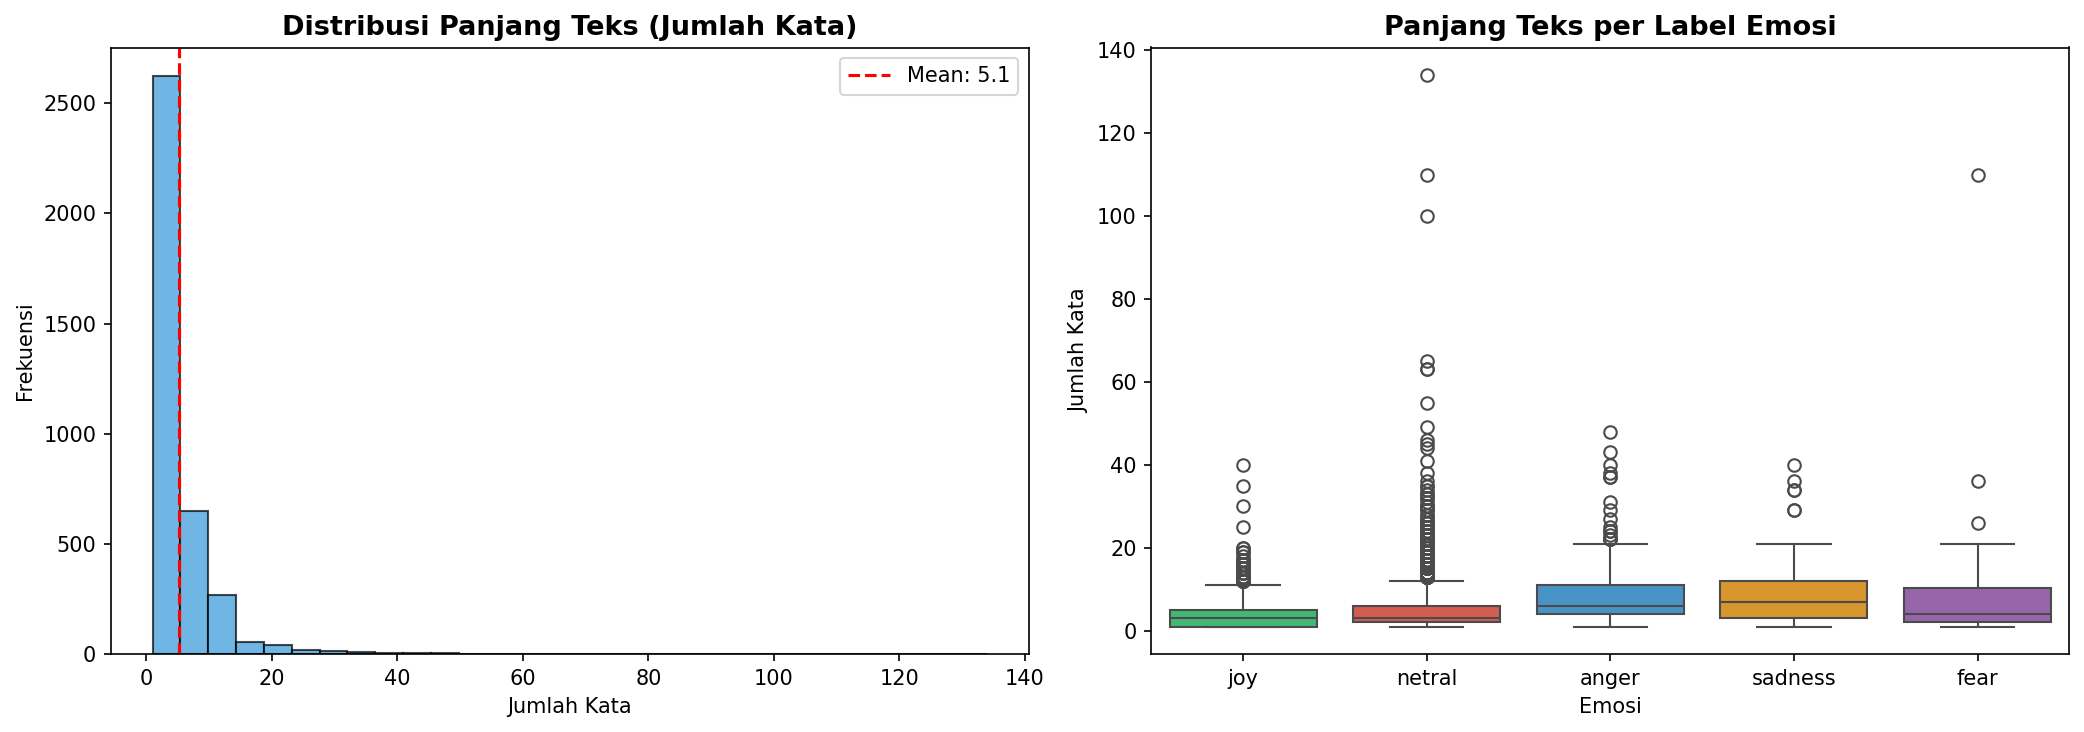
\includegraphics[width=0.95\textwidth]{fig2_text_length_analysis.png}
% \caption{Text length distribution and per\,class comparison.}
% \label{fig:textlen}
% \end{figure}


\begin{figure}[h]
\centering
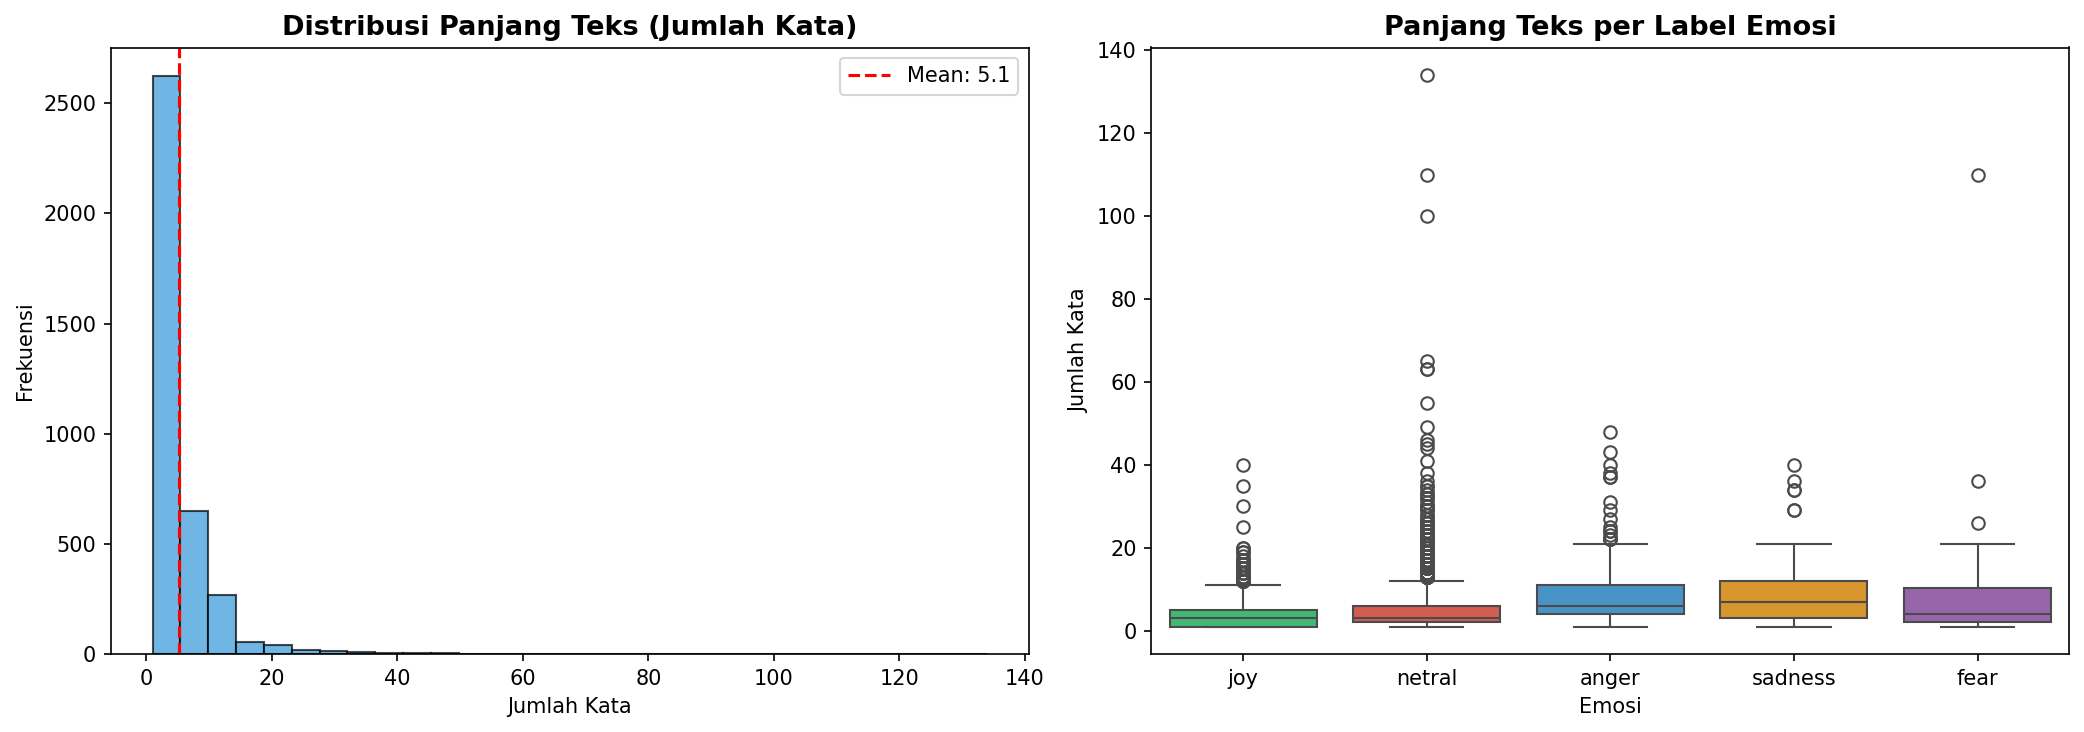
\includegraphics[width=0.95\textwidth]{fig2_text_length_analysis.png}
\caption{Text length analysis. Left: overall distribution of comment lengths (in words), showing that most comments are very short (median 3 words). Right: per\,class comparison revealing that negative emotion comments (anger, sadness, fear) tend to be longer than joy or neutral comments, suggesting that users write more when expressing dissatisfaction.}
\label{fig:textlen}
\end{figure}

\subsection{Preprocessing Pipeline}

The text was preprocessed through the following stages before being used in this project:

\begin{enumerate}[leftmargin=2em]
    \item \textbf{Text cleaning:} Removal of usernames, URLs, special characters, and numbers.
    \item \textbf{Normalization:} Conversion of slang and abbreviations to standard Indonesian (e.g., ``gak'' $\to$ ``tidak'', ``min'' $\to$ ``admin'').
    \item \textbf{Tokenization:} Splitting text into individual word tokens.
    \item \textbf{Stopword removal:} Removal of common Indonesian stopwords and domain\,specific noise words.
    \item \textbf{Stemming:} Reduction to root forms using Indonesian stemming rules (e.g., ``menyenangkan'' $\to$ ``senang'').
\end{enumerate}


The preprocessed text is stored in the \texttt{final\_text} column, which serves as the input for all subsequent analysis.

\newpage

\begin{figure}[h]
\centering
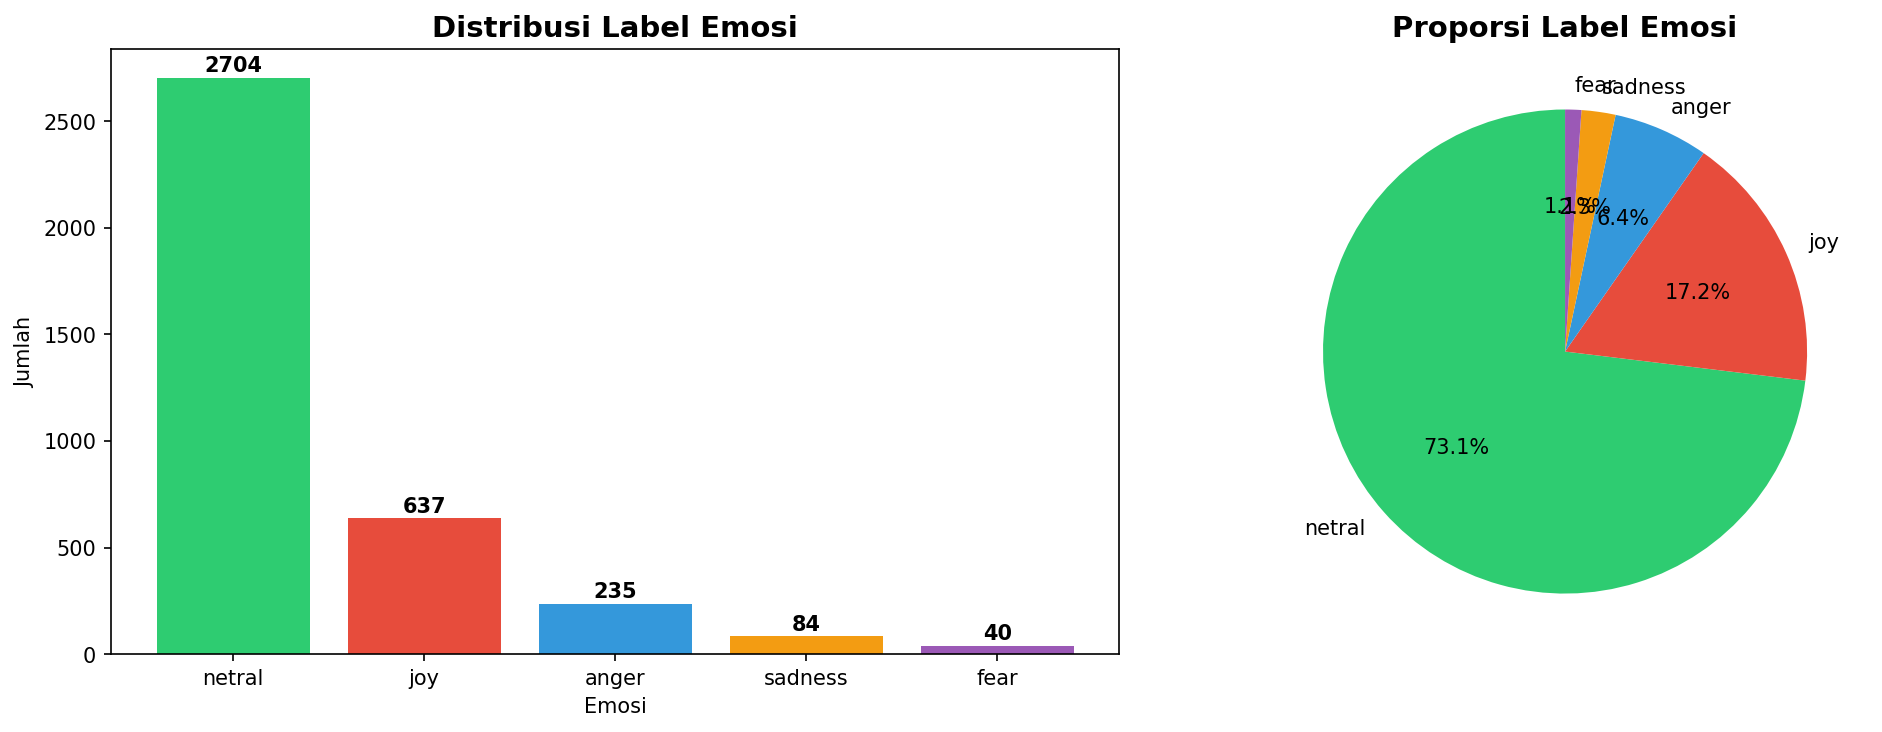
\includegraphics[width=0.95\textwidth]{fig1_label_distribution.png}
\caption{Original 5\,class emotion label distribution. Left: bar chart showing the severe imbalance, with neutral dominating at 2{,}704 samples. Right: pie chart illustrating that neutral comprises 73\% of all comments. The fear class (1.1\%) and sadness class (2.3\%) are barely visible, foreshadowing the classification difficulty documented in Section~\ref{sec:consolidation}.}
\label{fig:labeldist}
\end{figure}


\begin{figure}[h]
\centering
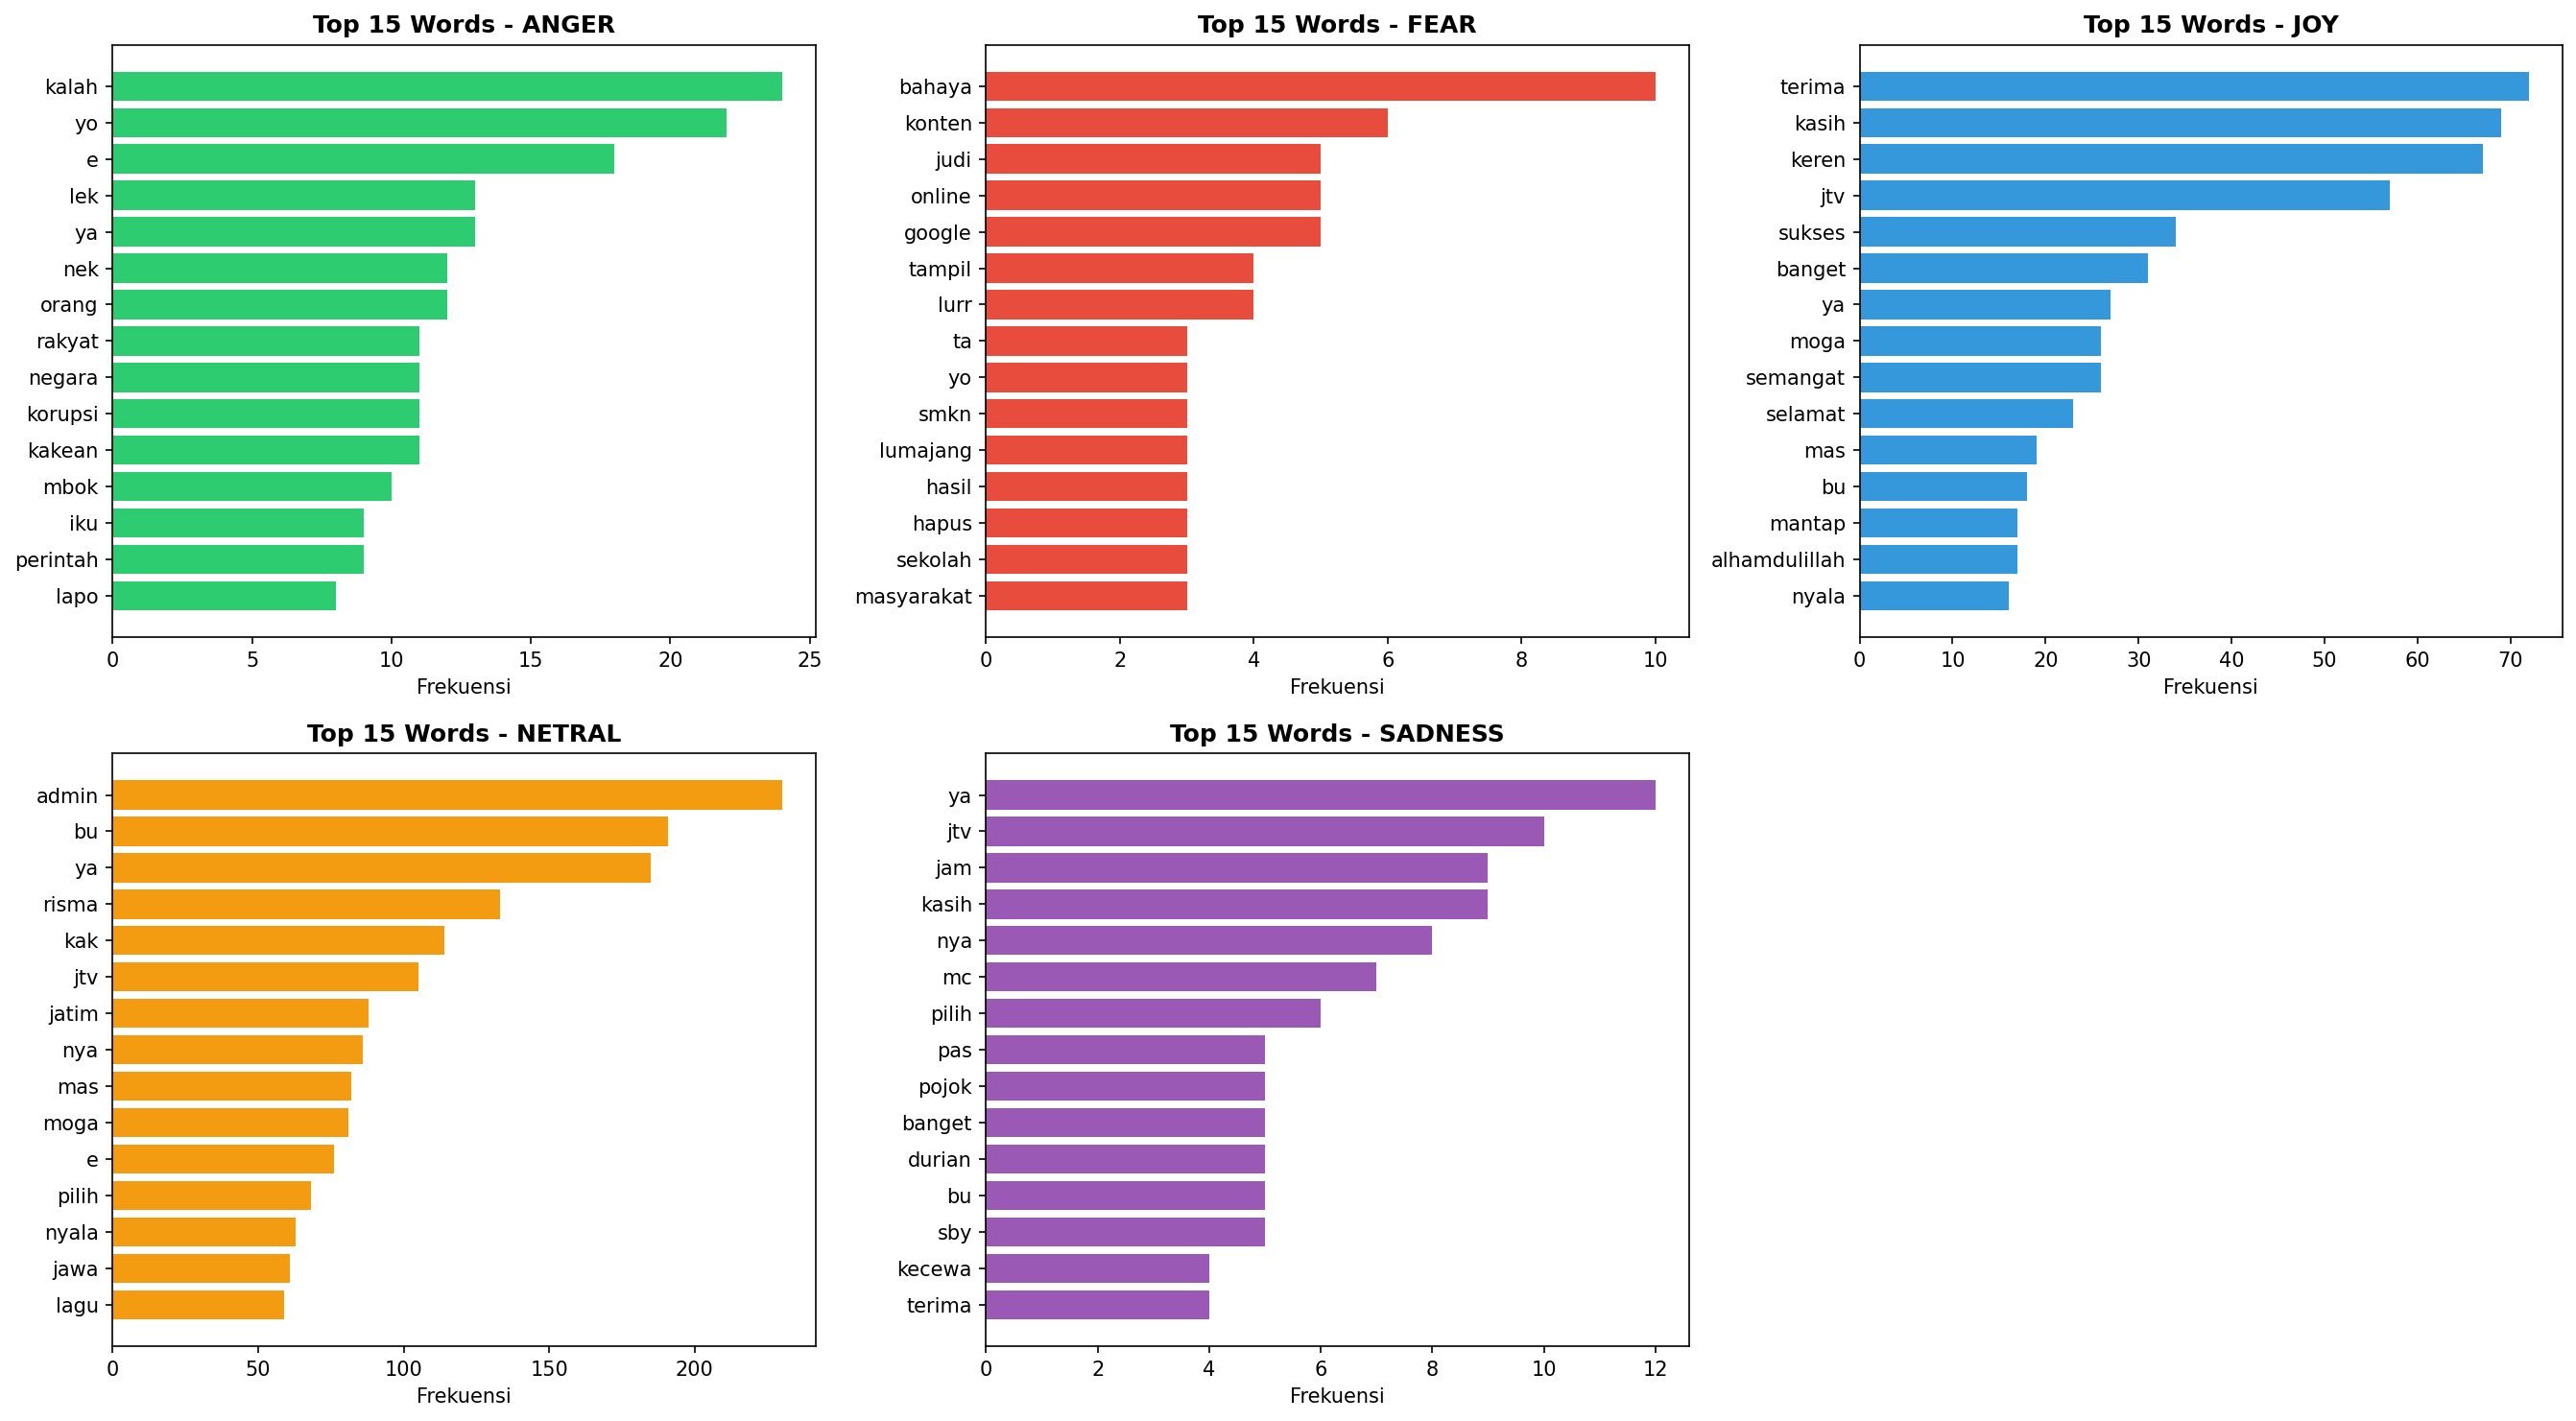
\includegraphics[width=0.95\textwidth]{fig3_word_frequency_per_emotion.png}
\caption{Top 15 most frequent words per emotion class. }
\label{fig:wordfreq}
\end{figure}

Each panel shows the most common words after preprocessing. Notice how joy comments are dominated by positive terms (``seru,'' ``keren,'' ``mantap''), anger comments contain critical terms (``teganya,'' ``buruk''), and neutral comments contain informational terms (``admin,'' ``syarat,'' ``info''). These word frequency patterns are exactly what TF\,IDF captures as numerical features.

\newpage
% ============================================================================
% SECTION 3: THE CLASS CONSOLIDATION DECISION
% ============================================================================
\section{A Critical Decision: From Five Classes to Three}
\label{sec:consolidation}

\subsection{The Problem with Five Classes}

This section documents a critical methodological decision that fundamentally shaped the project. In early experiments, we trained classifiers on all five original emotion classes. The results appeared promising at first: the overall accuracy reached 75.5\%. However, a closer examination of the per\,class classification report revealed a serious problem.

\begin{table}[h]
\centering
\caption{Per\,class results of the initial 5\,class classification attempt.}
\label{tab:5class-fail}
\begin{tabular}{lcccc}
\toprule
\textbf{Class} & \textbf{Precision} & \textbf{Recall} & \textbf{F1\,Score} & \textbf{Support (Test)} \\
\midrule
Anger & 0.29 & 0.04 & 0.07 & 47 \\
Fear & 0.00 & 0.00 & 0.00 & 8 \\
Joy & 0.66 & 0.31 & 0.43 & 127 \\
Neutral & 0.77 & 0.96 & 0.85 & 541 \\
Sadness & 0.00 & 0.00 & 0.00 & 17 \\
\midrule
\textbf{Macro Average} & 0.34 & 0.26 & 0.27 & 740 \\
\bottomrule
\end{tabular}
\end{table}

The model achieved \textbf{0.00 F1\,score on both fear and sadness}, and only 0.07 on anger. It was essentially predicting ``neutral'' for almost every comment. The 75.5\% accuracy was an illusion: a trivial baseline that always predicts ``neutral'' would achieve 73.1\% accuracy. The model had learned almost nothing beyond the majority class.

\begin{notebox}[Lesson Learned: Accuracy Can Be Misleading]
In imbalanced classification, accuracy is a poor metric. A model that correctly classifies the majority class while ignoring all minority classes can still achieve high accuracy. This is why \textbf{F1\,macro} (the unweighted average of per\,class F1 scores) is the primary metric in this project. F1\,macro treats all classes equally, regardless of their size, so a model that fails on any class will receive a low score.
\end{notebox}

\subsection{Root Cause Analysis}

The failure had a clear cause: \textbf{insufficient samples in the minority classes}. With only 40 fear samples total (approximately 8 in the test set) and 84 sadness samples (approximately 17 in the test set), no classification algorithm, no matter how sophisticated, can reliably learn to distinguish these classes. The problem is statistical, not algorithmic.

SMOTE (Synthetic Minority Oversampling Technique) was applied, but it inflated 40 fear samples to 2{,}163 synthetic samples. This created unrealistic synthetic examples that confused the model about the real test distribution.

\subsection{The Solution: Principled Class Consolidation}

Following standard practice in Indonesian emotion classification literature \citep{saputri2018emotion, junianto2024ensemble}, we consolidated the three negative emotion classes (anger, fear, sadness) into a single \textbf{negative} class. This decision is grounded in two justifications:

\begin{enumerate}[leftmargin=2em]
    \item \textbf{Statistical validity.} The consolidated ``negative'' class has 359 samples (approximately 72 in the test set), sufficient for meaningful classification and evaluation.

    \item \textbf{Semantic coherence.} Anger, fear, and sadness share negative emotional valence. From a business perspective, knowing that a comment expresses negative emotion is often more actionable than distinguishing between specific negative subtypes.
\end{enumerate}

\begin{table}[h]
\centering
\caption{Consolidated 3\,class emotion distribution.}
\label{tab:dist3}
\begin{tabular}{lrr}
\toprule
\textbf{Emotion} & \textbf{Count} & \textbf{Percentage} \\
\midrule
Neutral & 2{,}704 & 73.1\% \\
Joy & 637 & 17.2\% \\
Negative (anger + fear + sadness) & 359 & 9.7\% \\
\midrule
\textbf{Total} & \textbf{3{,}700} & \textbf{100\%} \\
\bottomrule
\end{tabular}
\end{table}

\begin{filebox}
\textbf{Code Reference:} The class consolidation is performed in \texttt{step2\_feature\_engineering.py}, in the section labeled ``Class Consolidation.'' The mapping is: joy $\to$ joy, neutral $\to$ neutral, anger $\to$ negative, fear $\to$ negative, sadness $\to$ negative. The script also generates \texttt{fig4a\_class\_consolidation.png} showing both distributions side by side.
\end{filebox}

\begin{figure}[h]
\centering
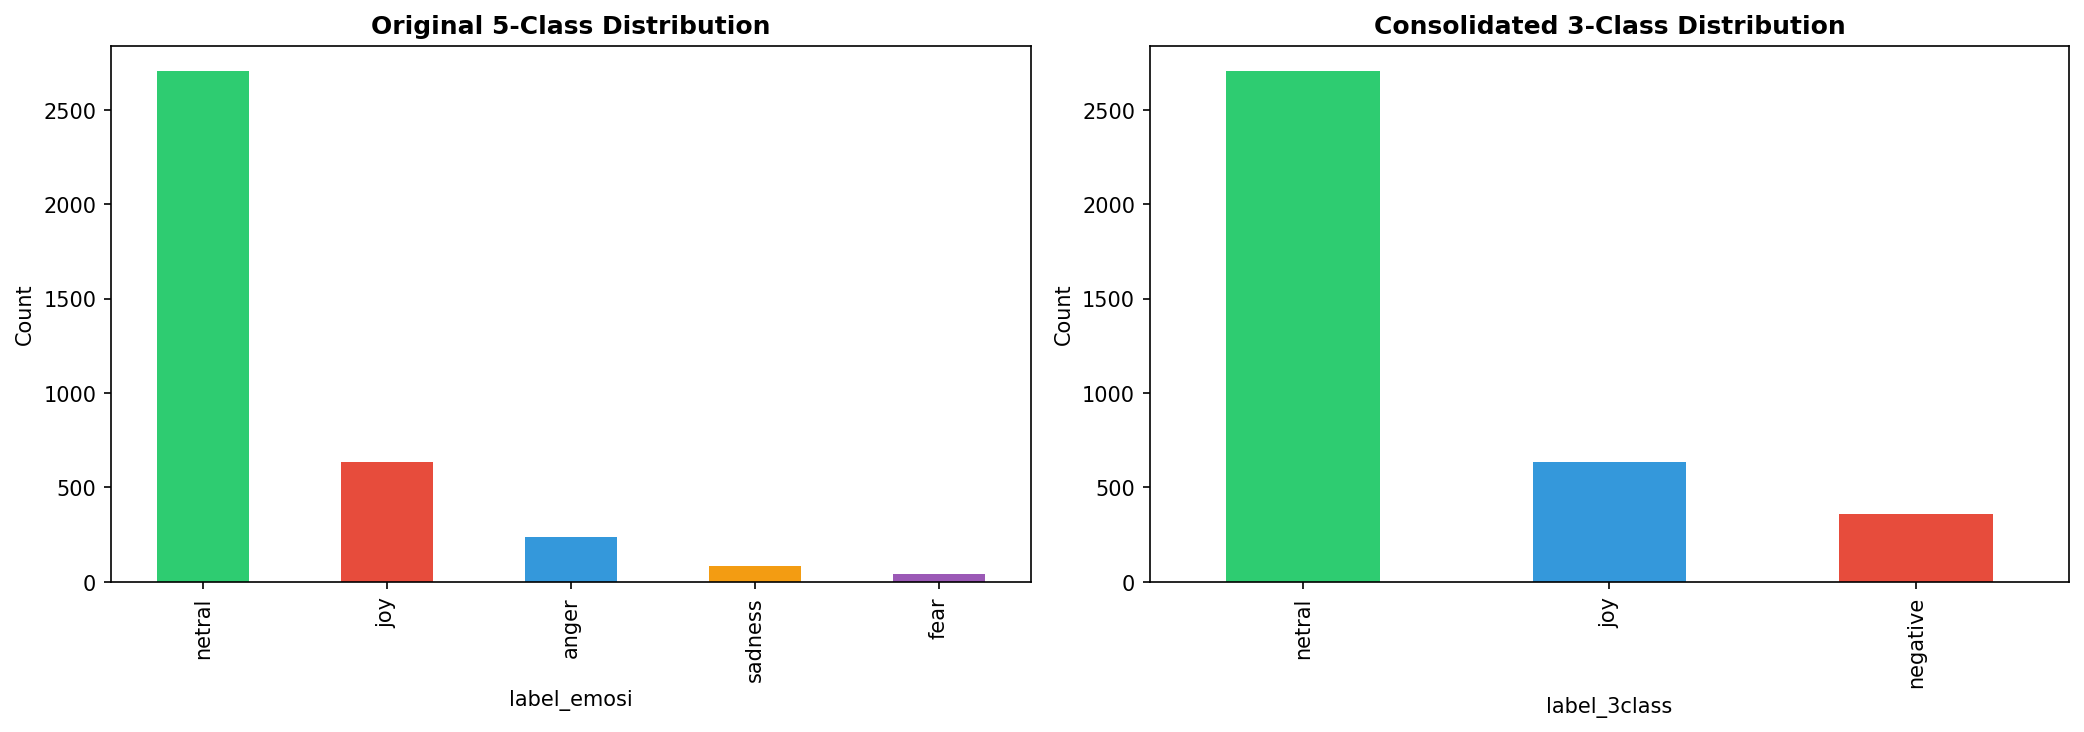
\includegraphics[width=0.95\textwidth]{fig4a_class_consolidation.png}
\caption{Class consolidation from 5 classes to 3. Left: original distribution with five classes. Right: consolidated distribution after merging anger, fear, and sadness into ``negative.'' The negative class now has 359 samples (9.7\%), providing sufficient data for reliable classification and evaluation.}
\label{fig:consolidation}
\end{figure}
 

% ============================================================================
% SECTION 4: THEORETICAL FOUNDATIONS
% ============================================================================
\section{Theoretical Foundations}
\label{sec:theory}

This section explains the key theories and techniques used in the project, including how each theory is applied in the code.

\subsection{TF\,--\,IDF: Turning Text into Numbers}

\subsubsection{The Theory}

Classifiers work with numbers, not text. The first step is to convert each comment into a numerical vector. \textbf{TF\,--\,IDF} (Term Frequency, Inverse Document Frequency) is a weighting scheme that assigns higher weights to words that are important within a document but rare across the corpus.

For a term $t$ in document $d$ from corpus $D$:
\begin{equation}
\text{TF\,--\,IDF}(t, d, D) = \text{TF}(t, d) \times \text{IDF}(t, D)
\end{equation}
where:
\begin{equation}
\text{TF}(t, d) = 1 + \log(\text{count of } t \text{ in } d)
\end{equation}
\begin{equation}
\text{IDF}(t, D) = \log\left(\frac{|D|}{|\{d \in D : t \in d\}|}\right)
\end{equation}

The \textbf{sublinear TF} formulation (using $1 + \log$ instead of raw count) dampens the effect of high\,frequency terms. A word appearing 10 times is not 10$\times$ more important than a word appearing once.

\subsubsection{How We Apply It}

In this project, TF\,--\,IDF is configured with the following parameters:

\begin{enumerate}[leftmargin=2em]
    \item \texttt{max\_features=5000}: Keep only the 5{,}000 most informative terms.
    \item \texttt{min\_df=3}: Ignore terms appearing in fewer than 3 documents (removes typos and very rare terms).
    \item \texttt{max\_df=0.90}: Ignore terms appearing in more than 90\% of documents (removes ubiquitous but uninformative terms).
    \item \texttt{ngram\_range=(1,2)}: Include both single words (unigrams) and word pairs (bigrams), capturing phrases like ``terima kasih'' (thank you) as single features.
    \item \texttt{sublinear\_tf=True}: Use the logarithmic TF formula above.
\end{enumerate}

The output is a sparse matrix of shape (3{,}700 $\times$ 1{,}556), where each row is one comment and each column is one TF\,--\,IDF feature. Since most comments do not contain most words, this matrix is approximately 99\% zeros (sparse).

\begin{filebox}
\textbf{Code Reference:} TF\,--\,IDF vectorization is performed in \texttt{step2\_feature\_engineering.py}, Section 3 (``TF\,--\,IDF Vectorization'').
\end{filebox}


\subsubsection{Intuition for Business Readers}
 
Think of TF\,IDF as a smart word counting system. If you asked a human analyst to summarize what makes an ``angry'' comment different from a ``joyful'' one, they would point to specific words: angry comments contain words like ``buruk'' (bad) or ``teganya'' (heartless), while joyful comments contain ``seru'' (fun) or ``mantap'' (great). TF\,IDF does exactly this automatically, but across thousands of comments simultaneously.
 
The ``IDF'' part is what makes it smart. The word ``admin'' appears in many comments of all emotions (users addressing the page administrator), so IDF gives it a low weight because it does not help distinguish emotions. The word ``teganya'' appears only in a few angry comments, so IDF gives it a high weight because it strongly signals a specific emotion. In business terms, TF\,IDF automatically identifies the words that matter for classification and ignores the noise.
 
\subsubsection{A Worked Example}
 
Consider two comments:
\begin{enumerate}[leftmargin=2em]
    \item ``seru banget'' (``so fun'') with label \textit{joy}
    \item ``buruk citra selenggara'' (``bad image organizer'') with label \textit{negative}
\end{enumerate}
 
After TF\,IDF processing, comment 1 gets high values for the ``seru'' and ``banget'' features and zero for ``buruk'' and ``citra.'' Comment 2 gets the reverse pattern. A classifier can then learn that high ``seru'' scores predict joy while high ``buruk'' scores predict negative emotion.


\subsection{Latent Semantic Analysis (LSA): Discovering Hidden Topics}

\subsubsection{The Theory}

The TF\,--\,IDF matrix is high\,dimensional (1{,}556 features) and sparse. \textbf{Latent Semantic Analysis} \citep{deerwester1990indexing} reduces this to a lower\,dimensional representation by discovering latent ``topics'' that capture the underlying semantic structure.

LSA works by applying \textbf{Truncated Singular Value Decomposition (SVD)} to the TF\,--\,IDF matrix $\mathbf{X}$:
\begin{equation}
\mathbf{X} \approx \mathbf{U}_k \boldsymbol{\Sigma}_k \mathbf{V}_k^T
\end{equation}
where $k$ is the number of topics (dimensions to retain), $\mathbf{U}_k$ contains the document\,topic relationships, $\boldsymbol{\Sigma}_k$ contains the topic strengths, and $\mathbf{V}_k$ contains the term\,topic relationships.

The transformed data $\mathbf{X}_{\text{LSA}} = \mathbf{U}_k \boldsymbol{\Sigma}_k$ gives each document a $k$\,dimensional vector where each dimension represents a latent topic.

\subsubsection{Why LSA Helps}

LSA provides three benefits:
\begin{enumerate}[leftmargin=2em]
    \item \textbf{Dimensionality reduction:} Reduces 1{,}556 sparse features to $k$ dense features (e.g., 25), making classifiers faster and less prone to overfitting.
    \item \textbf{Semantic smoothing:} Groups related terms together. Even if one comment says ``keren'' (cool) and another says ``mantap'' (great), they may map to the same topic.
    \item \textbf{Noise reduction:} Removes the low\,variance dimensions that often correspond to noise.
\end{enumerate}

\subsubsection{The Granularity Question}

A fundamental question in LSA is: \textit{how many topics ($k$) should we use?} Too few topics ($k=5$) oversimplifies the data, collapsing distinct concepts into the same dimension. Too many topics ($k=100$) retains noise and may not improve classification.

This project systematically tests $k \in \{5, 10, 25, 50, 100\}$ and measures classification performance at each level. This \textbf{granularity analysis} is a core contribution of the research.

\begin{notebox}[Explained Variance at Each Granularity]

The cumulative explained variance ratio increases with $k$: $k=5$ captures 6.2\%, $k=10$ captures 10.0\%, $k=25$ captures 17.2\%, $k=50$ captures 25.5\%, and $k=100$ captures 36.7\% of the total variance. However, more variance does not always mean better classification, because some of that variance may represent noise rather than emotion\,discriminative information.

\end{notebox}


\begin{figure}[h]
\centering
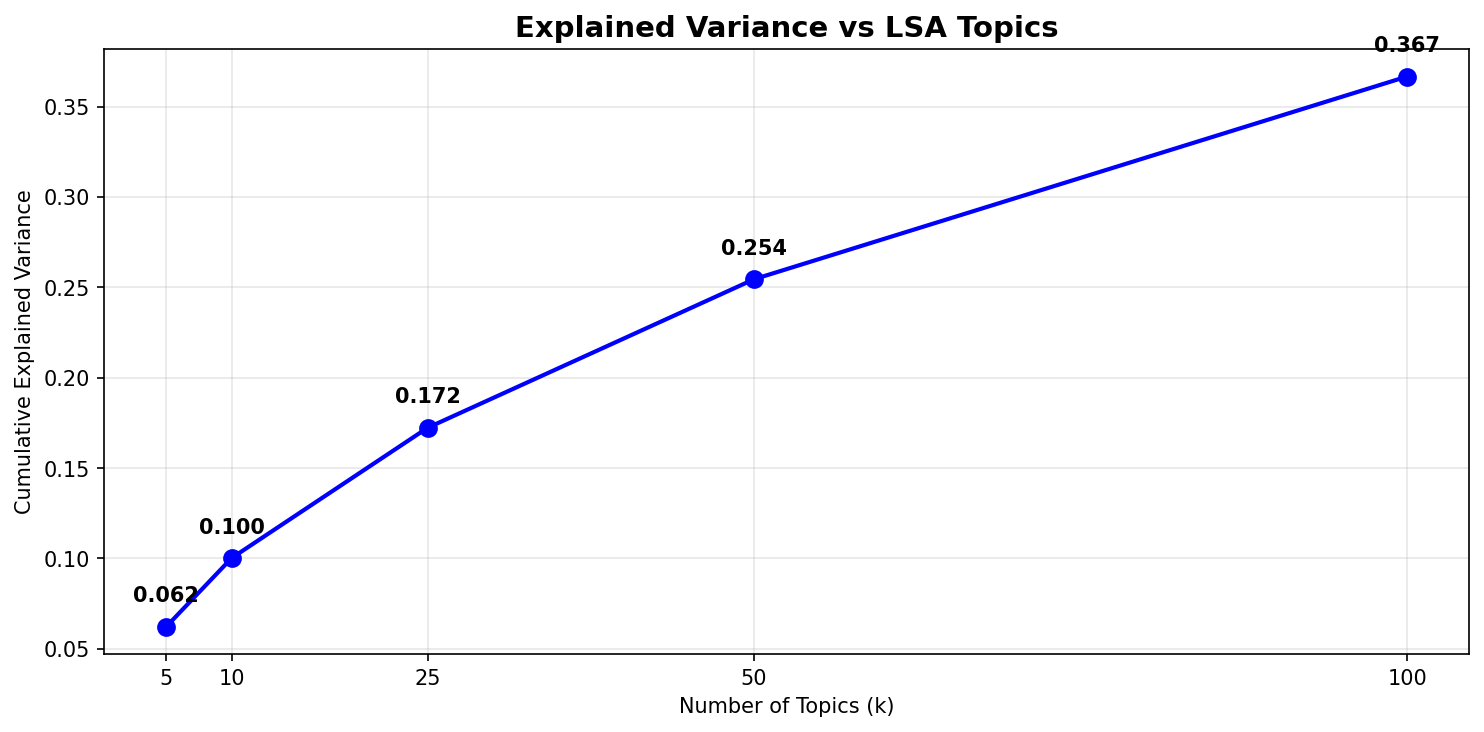
\includegraphics[width=0.85\textwidth]{fig4_lsa_explained_variance.png}
\caption{Cumulative explained variance ratio as a function of the number of LSA topics ($k$). At $k=5$, only 6.2\% of the variance is captured, while $k=100$ captures 36.7\%. However, classification performance does not follow variance monotonically: the best F1\,macro occurs at $k=25$ (17.2\% variance), suggesting that higher dimensions introduce noise rather than useful signal for emotion classification.}
\label{fig:lsa-ev}
\end{figure}

\subsubsection{Multi\,Topic Feature Concatenation}

We also test whether combining LSA features from multiple granularities improves classification. The idea is to concatenate the feature vectors: $[\text{LSA}_{k=5} | \text{LSA}_{k=10} | \text{LSA}_{k=25} | \text{LSA}_{k=50} | \text{LSA}_{k=100}]$, producing a 190\,dimensional feature vector that captures both coarse and fine semantic structure.

\begin{filebox}
\textbf{Code Reference:} All LSA computations and multi\,topic concatenation are in \texttt{step2\_feature\_engineering.py}, Sections 4 and 5. The explained variance plot is saved as \texttt{fig4\_lsa\_explained\_variance.png}.
\end{filebox}


\subsubsection{Intuition for Business Readers}
 
Imagine you have a spreadsheet with 3{,}700 rows (comments) and 1{,}556 columns (words). Most cells are zero because most comments do not contain most words. LSA compresses this spreadsheet from 1{,}556 columns down to just 25 columns (when $k=25$), where each new column represents a ``topic'' or theme rather than a single word.
 
For example, Topic 1 might capture ``political discussion'' (combining words like ``risma,'' ``jatim,'' ``bupati''), while Topic 5 might capture ``positive entertainment reactions'' (combining ``keren,'' ``banget,'' ``seru''). Instead of tracking 1{,}556 individual words, the classifier now works with 25 meaningful themes, which is both faster and more accurate because it groups related words together.
 
This is like the difference between filing documents by every individual word they contain (thousands of categories) versus filing them by topic (a few dozen categories). The topic\,based filing system is more useful even though it throws away some detail.
 
\subsubsection{Visualizing the Topics}
 
The top terms for each of the 10 topics (at $k=10$) reveal clear thematic clusters in the Instagram comments:
 
\begin{table}[h]
\centering
\caption{Top terms per LSA topic ($k=10$), showing thematic clusters.}
\label{tab:topics}
\small
\begin{tabular}{cl}
\toprule
\textbf{Topic} & \textbf{Top Terms (Thematic Interpretation)} \\
\midrule
1 & risma, bu, bu risma, jatim, nyala \textit{(Political discussion)} \\
2 & admin, kasih, terima, terima kasih, kak \textit{(Gratitude/requests)} \\
3 & nyala, lur, ning, nyala lur, abang \textit{(Community engagement)} \\
4 & admin, request, lagu, request lagu, undang \textit{(Song/show requests)} \\
5 & keren, banget, keren banget, kali, nih \textit{(Positive reactions)} \\
6 & kak, ya, atas, like, post atas \textit{(Engagement actions)} \\
7 & lur, mas, luluk, jatim, bu luluk \textit{(Political figures)} \\
8 & lur, ya, risma, jtv, bu risma \textit{(JTV/political)} \\
9 & ya, jtv, sukses, jatim, moga, selamat \textit{(Well wishes)} \\
10 & jatim, kak, pilih, maju, jatim maju \textit{(Regional pride)} \\
\bottomrule
\end{tabular}
\end{table}
 
Notice how Topics 5 and 9 (positive reactions, well wishes) align with the ``joy'' emotion, while Topics 1 and 7 (political discussion) often correlate with ``negative'' or ``neutral'' emotions. LSA discovers these patterns automatically without any supervision.

\subsection{Handling Class Imbalance: SMOTE}

\subsubsection{The Theory}

When one class has far more samples than others, classifiers tend to favor the majority class because that minimizes overall error. \textbf{SMOTE} (Synthetic Minority Oversampling Technique) \citep{chawla2002smote} addresses this by generating synthetic samples for minority classes.

For each minority sample $\mathbf{x}$:
\begin{enumerate}[leftmargin=2em]
    \item Find its $k$ nearest neighbors in the same class (we use $k=3$).
    \item Randomly select one neighbor $\hat{\mathbf{x}}$.
    \item Create a new synthetic sample: $\mathbf{x}_{\text{new}} = \mathbf{x} + \lambda(\hat{\mathbf{x}} - \mathbf{x})$ where $\lambda \sim \text{Uniform}(0,1)$.
\end{enumerate}

This creates new samples that lie on the line segment between existing minority samples, expanding the decision boundary for the minority class.

\subsubsection{How We Apply It}

SMOTE is applied \textbf{after} the train/test split and \textbf{only on the training set} to prevent data leakage. In our 3\,class setting, the training distribution before SMOTE is: joy (510), negative (287), neutral (2{,}163). After SMOTE, all classes have 2{,}163 samples.


\subsubsection{Intuition for Business Readers}
 
Imagine you are training a new employee to sort customer feedback into ``happy,'' ``unhappy,'' and ``neutral.'' You give them 100 training examples, but 73 are neutral, 17 are happy, and only 10 are unhappy. The employee quickly learns that guessing ``neutral'' most of the time gets them a high score (73\% correct). They barely learn to recognize unhappy feedback because they see so few examples.
 
SMOTE solves this by creating additional training examples for the underrepresented categories. It does not simply copy existing examples (which would cause the model to memorize rather than generalize). Instead, it creates new examples that are \textit{similar but not identical} to existing ones, by interpolating between real examples. After SMOTE, the employee sees equal numbers of happy, unhappy, and neutral examples, and learns to recognize all three patterns.
 
The trade\,off is that some of the synthetic ``unhappy'' examples may not perfectly represent real unhappy feedback, causing the employee to occasionally misclassify neutral feedback as unhappy. This is exactly the accuracy vs.\ F1\,macro trade\,off we observe in our experiments.

\begin{notebox}[SMOTE Trade\,off: A Key Finding]
Our experiments reveal a consistent trade\,off: SMOTE improves F1\,macro (the main metric for imbalanced classification) by approximately +2\% on average, but decreases accuracy by approximately $-$12\% on average. This happens because SMOTE increases recall on minority classes (the model correctly identifies more emotional comments) but also increases false positives (some neutral comments are incorrectly classified as emotional). We quantify this trade\,off for each LSA granularity in Section~\ref{sec:results}.
\end{notebox}

\subsection{Classification Models}

\subsubsection{Random Forest}

\textbf{Random Forest} \citep{breiman2001random} is an ensemble of decision trees, each trained on a random subset of data and features. The final prediction is the majority vote across all trees.

In our configuration: 200 trees (\texttt{n\_estimators=200}), maximum depth 20, and \texttt{class\_weight='balanced'} (which automatically adjusts class weights inversely proportional to class frequency).

\subsubsection{Support Vector Machine (SVM)}

\textbf{SVM} \citep{cortes1995support} finds the hyperplane that maximally separates classes in a high\,dimensional space. With the RBF (Radial Basis Function) kernel, it can capture nonlinear decision boundaries.

Our configuration uses \texttt{C=10} (regularization), \texttt{gamma='scale'}, \texttt{class\_weight='balanced'}, and wraps SVM inside a \texttt{StandardScaler} pipeline because SVM is sensitive to feature scale. This scaling is especially important when using multi\,topic concatenated features where different LSA granularities have different variance profiles.

\subsubsection{XGBoost}

\textbf{XGBoost} \citep{chen2016xgboost} (Extreme Gradient Boosting) builds trees sequentially, where each tree corrects the errors of the previous ones. It is known for strong performance on tabular data.

Our configuration: 200 trees, maximum depth 6, learning rate 0.1.

\subsubsection{Stacking Ensemble}

\textbf{Stacking} \citep{wolpert1992stacked} is a meta\,learning technique that combines multiple base classifiers by training a second\,level ``meta\,learner'' on their predictions. The idea is that different classifiers make different types of errors, and a meta\,learner can learn which classifier to trust in which situations.

Our stacking architecture:
\begin{enumerate}[leftmargin=2em]
    \item \textbf{Base learners:} Random Forest, SVM, XGBoost (each trained on the full training data).
    \item \textbf{Meta\,feature generation:} 5\,fold cross\,validation generates out\,of\,fold probability predictions. Each base learner produces 3 probabilities (one per class), giving $3 \times 3 = 9$ meta\,features.
    \item \textbf{Meta\,learner:} Logistic Regression trained on the 9 meta\,features to produce the final prediction.
\end{enumerate}

\begin{notebox}[Why Stacking Over Simple Voting]
Stacking learns the \textit{optimal weighting} of base classifiers, whereas voting treats all classifiers equally. In our experiments, stacking consistently outperforms all individual classifiers across granularities, demonstrating the value of this learned combination.
\end{notebox}

\subsubsection{Intuition for Business Readers}
 
Think of stacking as assembling a panel of expert advisors. Each expert (Random Forest, SVM, XGBoost) has different strengths:
 
\begin{enumerate}[leftmargin=2em]
    \item \textbf{Random Forest} is like a conservative committee that votes. It rarely makes extreme mistakes but may miss subtle patterns.
    \item \textbf{SVM} is like a geometry expert who draws precise boundaries between categories. It excels when categories are well separated but struggles with overlapping groups.
    \item \textbf{XGBoost} is like an iterative editor who keeps refining. It learns from the mistakes of previous rounds and gradually improves.
\end{enumerate}
 
The meta\,learner (Logistic Regression) acts as the \textbf{chairperson} who has observed all three experts over many cases and learned when each expert is most trustworthy. For some comments, the chairperson trusts SVM more; for others, XGBoost. This learned weighting is more effective than simply taking a majority vote.
 
\begin{figure}[h]
\centering
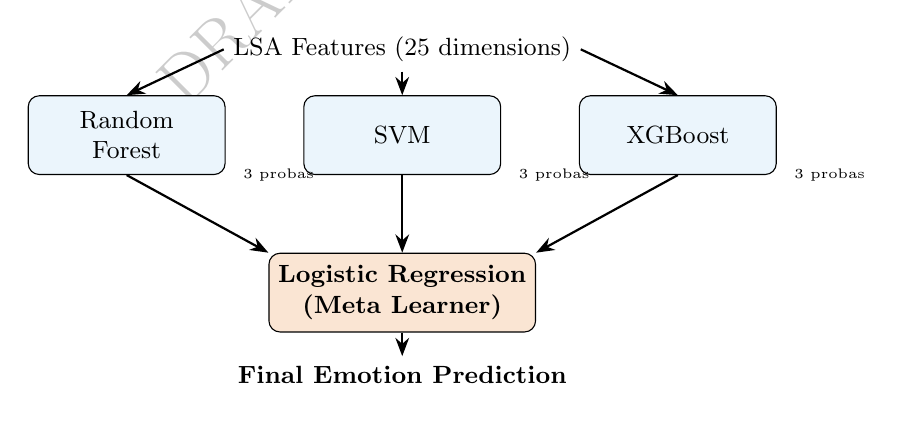
\begin{tikzpicture}[
    box/.style={draw, rounded corners, fill=lightblue, minimum width=2.5cm, minimum height=1cm, align=center, font=\small},
    meta/.style={draw, rounded corners, fill=accentorange!20, minimum width=3cm, minimum height=1cm, align=center, font=\small\bfseries},
    arr/.style={-{Stealth}, thick}
]
\node[box] (rf) at (0,0) {Random\\Forest};
\node[box] (svm) at (3.5,0) {SVM};
\node[box] (xgb) at (7,0) {XGBoost};
 
\node[font=\small, above=0.3cm of svm] (input) {LSA Features (25 dimensions)};
\draw[arr] (input.west) -- (rf.north);
\draw[arr] (input) -- (svm.north);
\draw[arr] (input.east) -- (xgb.north);
 
\node[meta] (meta) at (3.5,-2) {Logistic Regression\\(Meta Learner)};
\draw[arr] (rf.south) -- (meta.north west);
\draw[arr] (svm.south) -- (meta.north);
\draw[arr] (xgb.south) -- (meta.north east);
 
\node[font=\small\bfseries, below=0.3cm of meta] (output) {Final Emotion Prediction};
\draw[arr] (meta.south) -- (output.north);
 
\node[font=\tiny, right=0.1cm of rf.south east] {3 probas};
\node[font=\tiny, right=0.1cm of svm.south east] {3 probas};
\node[font=\tiny, right=0.1cm of xgb.south east] {3 probas};
\end{tikzpicture}
\caption{Stacking ensemble architecture. Each base learner produces 3 class probabilities, and the meta learner combines all 9 values into a final prediction.}
\label{fig:stacking-arch}
\end{figure}

\begin{filebox}
\textbf{Code Reference:} All models and experiments are defined and executed in \texttt{step3\_experiments.py}. The stacking ensemble uses scikit\,learn's \texttt{StackingClassifier} with 5\,fold cross\,validation and probability\,based stacking.
\end{filebox}

\newpage
% ============================================================================
% SECTION 5: THE CODE PIPELINE
% ============================================================================
\section{The Code Pipeline: What Each Script Does}
\label{sec:pipeline}

This section maps the complete pipeline, script by script, so readers can understand exactly what happens at each stage and reproduce all results.

\subsection{Overview}

The project consists of four Python scripts, executed in order:


\begin{table}[h]
\centering
\caption{Project scripts and their roles.}
\label{tab:scripts}
\begin{tabular}{p{4.5cm}p{9cm}}
\toprule
\textbf{Script} & \textbf{Purpose} \\
\midrule
% Using \url{} inside the first column allows LaTeX to break the text at underscores
\url{step1_eda_preprocessing.py} & Loads the raw CSV, cleans missing values, computes label distribution and text statistics, generates EDA figures. \\ \addlinespace
\url{step2_feature_engineering.py} & Consolidates 5 classes to 3, builds TF--IDF features, computes LSA at 5 granularities, creates multi-topic features, performs train/test split. \\ \addlinespace
\url{step3_experiments.py} & Runs all 28 experiments: individual models, stacking ensembles, TF--IDF baseline, SMOTE vs.\ no-SMOTE comparison, multi-topic vs.\ single-topic. \\ \addlinespace
\url{step4_evaluation.py} & Generates all 13 publication figures, 7 tables (with LaTeX versions), and the final publication summary. \\
\bottomrule
\end{tabular}
\end{table}



\subsection{Step 1: Exploratory Data Analysis}

\texttt{step1\_eda\_preprocessing.py} performs:

\begin{enumerate}[leftmargin=2em]
    \item Loads the dataset from \texttt{preprocessing\_instagram\_xlsx\_-\_JASMINE.csv}.
    \item Drops rows with missing \texttt{final\_text} or \texttt{label\_emosi} (2 rows each).
    \item Computes and prints the label distribution, imbalance ratio (67.6:1), and text length statistics per class.
    \item Generates three figures: label distribution (Figure 1), text length analysis (Figure 2), and word frequency per emotion (Figure 3).
    \item Saves the cleaned dataset to \texttt{outputs/data\_cleaned.csv}.
\end{enumerate}

\subsection{Step 2: Feature Engineering}

\texttt{step2\_feature\_engineering.py} performs:

\begin{enumerate}[leftmargin=2em]
    \item Loads the cleaned dataset.
    \item \textbf{Class consolidation:} Maps anger, fear, sadness $\to$ ``negative'', producing 3 classes.
    \item \textbf{Label encoding:} Converts string labels to integers (joy=0, negative=1, neutral=2).
    \item \textbf{TF\,--\,IDF:} Transforms text into a 3{,}700 $\times$ 1{,}556 sparse matrix.
    \item \textbf{LSA:} Applies TruncatedSVD at $k \in \{5, 10, 25, 50, 100\}$, saving each result.
    \item \textbf{Multi\,topic concatenation:} Stacks all LSA features into a 190\,dimensional matrix.
    \item \textbf{Train/test split:} 80/20 stratified split, preserving class proportions.
    \item Saves all feature matrices, label arrays, and the label encoder to the \texttt{outputs/} directory.
\end{enumerate}

\subsection{Step 3: Experiments}

\texttt{step3\_experiments.py} is the core experimental script. It runs six experiment groups:

\begin{enumerate}[leftmargin=2em]
    \item \textbf{3A: Individual Models + SMOTE.} Trains RF, SVM, XGB separately at each $k$ using SMOTE\,augmented data. This produces 15 results (3 models $\times$ 5 granularities).

    \item \textbf{3B: Stacking + SMOTE.} Trains the stacking ensemble at each $k$ using SMOTE. This produces 5 results and identifies the \textbf{optimal granularity} (k=25, F1\,macro=0.5087).

    \item \textbf{3C: TF\,--\,IDF Baseline.} Trains stacking on raw TF\,--\,IDF features (no LSA) to confirm that LSA adds value.

    \item \textbf{3D: Stacking without SMOTE.} Repeats 3B without SMOTE oversampling, enabling a controlled comparison of SMOTE effectiveness.

    \item \textbf{3E: Multi\,Topic + SMOTE.} Trains stacking on the 190\,dimensional concatenated features to test whether multi\,granularity helps.

    \item \textbf{3F: Multi\,Topic without SMOTE.} Completes the comparison matrix.
\end{enumerate}

After all experiments, the script saves \texttt{all\_results.csv} (28 rows, one per experiment), \texttt{smote\_analysis.csv} (paired SMOTE comparison), and the predictions for the best model.

\subsection{Step 4: Evaluation and Visualization}

\texttt{step4\_evaluation.py} generates all publication materials:

\begin{enumerate}[leftmargin=2em]
    \item Loads all experiment results and the best model's predictions.
    \item Generates 9 additional figures (Figures 5 through 13).
    \item Generates 7 tables as both CSV and LaTeX files.
    \item Prints the complete \texttt{PUBLICATION SUMMARY} with all key numbers.
\end{enumerate}

\subsection{Running the Pipeline}

\begin{filebox}
\textbf{Prerequisites:} Python 3.8+ with packages listed in \texttt{requirements.txt}: pandas, numpy, scikit\,learn, xgboost, imbalanced\,learn, matplotlib, seaborn, scipy.

\textbf{To run:}
\begin{enumerate}[leftmargin=2em]
    \item Place \texttt{preprocessing\_instagram\_xlsx\_-\_JASMINE.csv} in the project directory.
    \item Install dependencies: \texttt{pip install -r requirements.txt}
    \item Run all steps: \texttt{python run\_all.py} (approximately 15 to 20 minutes).
    \item Alternatively, run each step individually in order.
\end{enumerate}
\end{filebox}

% ============================================================================
% SECTION 6: RESULTS AND ANALYSIS
% ============================================================================
\section{Results and Analysis}
\label{sec:results}

\subsection{Finding 1: Optimal LSA Granularity is k=25}

The central finding of this research is that \textbf{k=25 LSA topics} produces the best emotion classification performance when combined with stacking ensemble and SMOTE.

\begin{table}[h]
\centering
\caption{Stacking ensemble performance across LSA granularities (with SMOTE).}
\label{tab:granularity}
\begin{tabular}{lcccc}
\toprule
\textbf{Model} & \textbf{Accuracy} & \textbf{F1\,Weighted} & \textbf{F1\,Macro} & \textbf{Time (s)} \\
\midrule
Stacking k=5 & 0.5946 & 0.6182 & 0.4441 & 20 \\
Stacking k=10 & 0.6297 & 0.6484 & 0.4937 & 20 \\
\textbf{Stacking k=25} & \textbf{0.6554} & \textbf{0.6669} & \textbf{0.5087} & \textbf{21} \\
Stacking k=50 & 0.6581 & 0.6654 & 0.4995 & 24 \\
Stacking k=100 & 0.6608 & 0.6629 & 0.4801 & 38 \\
\bottomrule
\end{tabular}
\end{table}

The pattern is clear: F1\,macro increases from k=5 to k=25, peaks at k=25, then decreases. This suggests k=25 provides the best balance between capturing enough semantic structure and avoiding noise.

\begin{notebox}[Why Accuracy Increases While F1\,Macro Decreases After k=25]
At $k=50$ and $k=100$, accuracy is slightly higher (0.6581, 0.6608) than at $k=25$ (0.6554). But F1\,macro is lower. This means the larger models are better at classifying neutral comments (the majority class) but worse at classifying emotional comments. Since our business goal is to detect emotions, F1\,macro is the more relevant metric.
\end{notebox}

% --- INSERT FIGURE HERE ---
% \begin{figure}[h]
% \centering
% 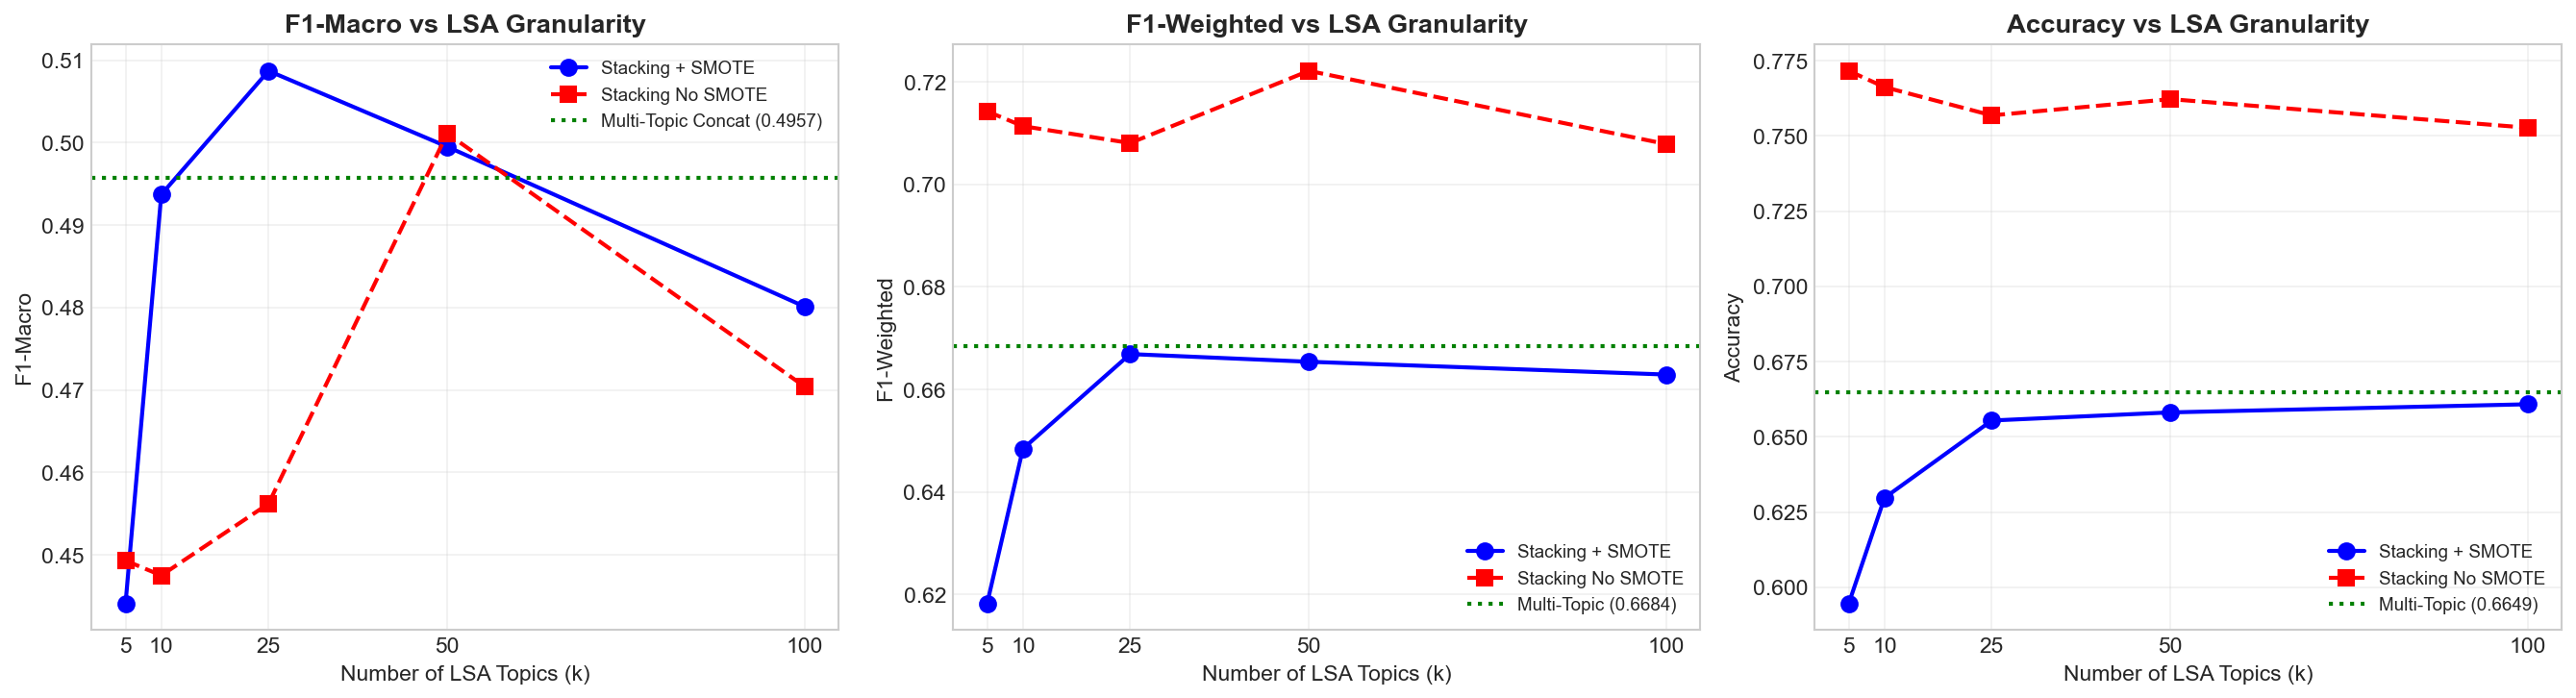
\includegraphics[width=\textwidth]{fig5_granularity_comparison.png}
% \caption{F1\,Macro, F1\,Weighted, and Accuracy across LSA granularities.}
% \label{fig:granularity}
% \end{figure}


\begin{figure}[h]
\centering
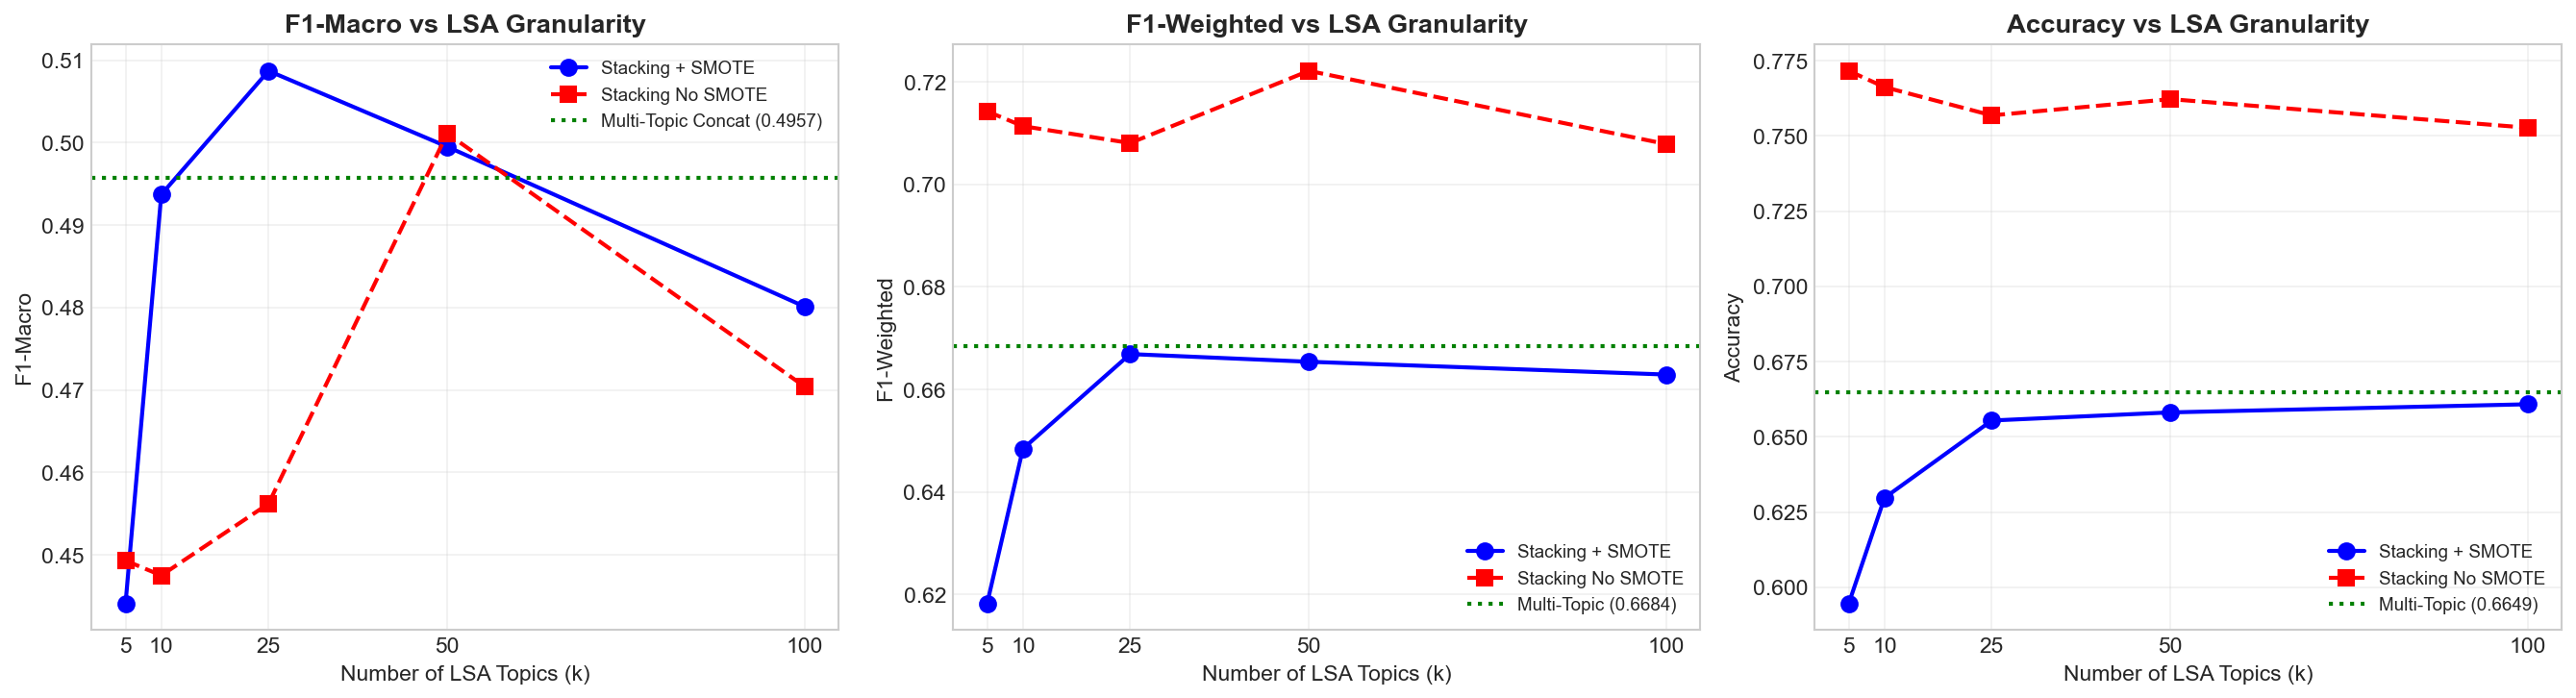
\includegraphics[width=\textwidth]{fig5_granularity_comparison.png}
\caption{Performance metrics across LSA granularities. Left: F1\,macro peaks at $k=25$ for the SMOTE configuration, confirming that 25 topics provide the best balance of signal and noise. Center: F1\,weighted shows a similar but less pronounced peak. Right: accuracy increases monotonically with $k$ but this is misleading because it primarily reflects better neutral classification, not better emotion detection. The green dotted line shows the multi\,topic concatenation result for comparison.}
\label{fig:granularity}
\end{figure}

\subsection{Finding 2: Stacking Outperforms Individual Models}

Across all granularities, the stacking ensemble consistently outperforms individual classifiers on F1\,macro.

\begin{table}[h]
\centering
\caption{Best individual model vs.\ stacking at each granularity (F1\,macro).}
\label{tab:indiv-vs-stack}
\begin{tabular}{lccc}
\toprule
\textbf{Granularity} & \textbf{Best Individual} & \textbf{Stacking} & \textbf{Difference} \\
\midrule
k=5 & XGB (0.4557) & 0.4441 & $-$0.0116 \\
k=10 & XGB (0.4844) & 0.4937 & +0.0093 \\
k=25 & RF (0.5070) & 0.5087 & +0.0017 \\
k=50 & XGB (0.5004) & 0.4995 & $-$0.0009 \\
k=100 & XGB (0.5116) & 0.4801 & $-$0.0315 \\
\bottomrule
\end{tabular}
\end{table}

The stacking advantage is most consistent at the optimal granularity (k=25), while individual XGBoost can occasionally outperform stacking at other k values. This reinforces that k=25 is the ``sweet spot'' where the ensemble can most effectively combine diverse classifiers.

% --- INSERT FIGURE HERE ---
% \begin{figure}[h]
% \centering
% 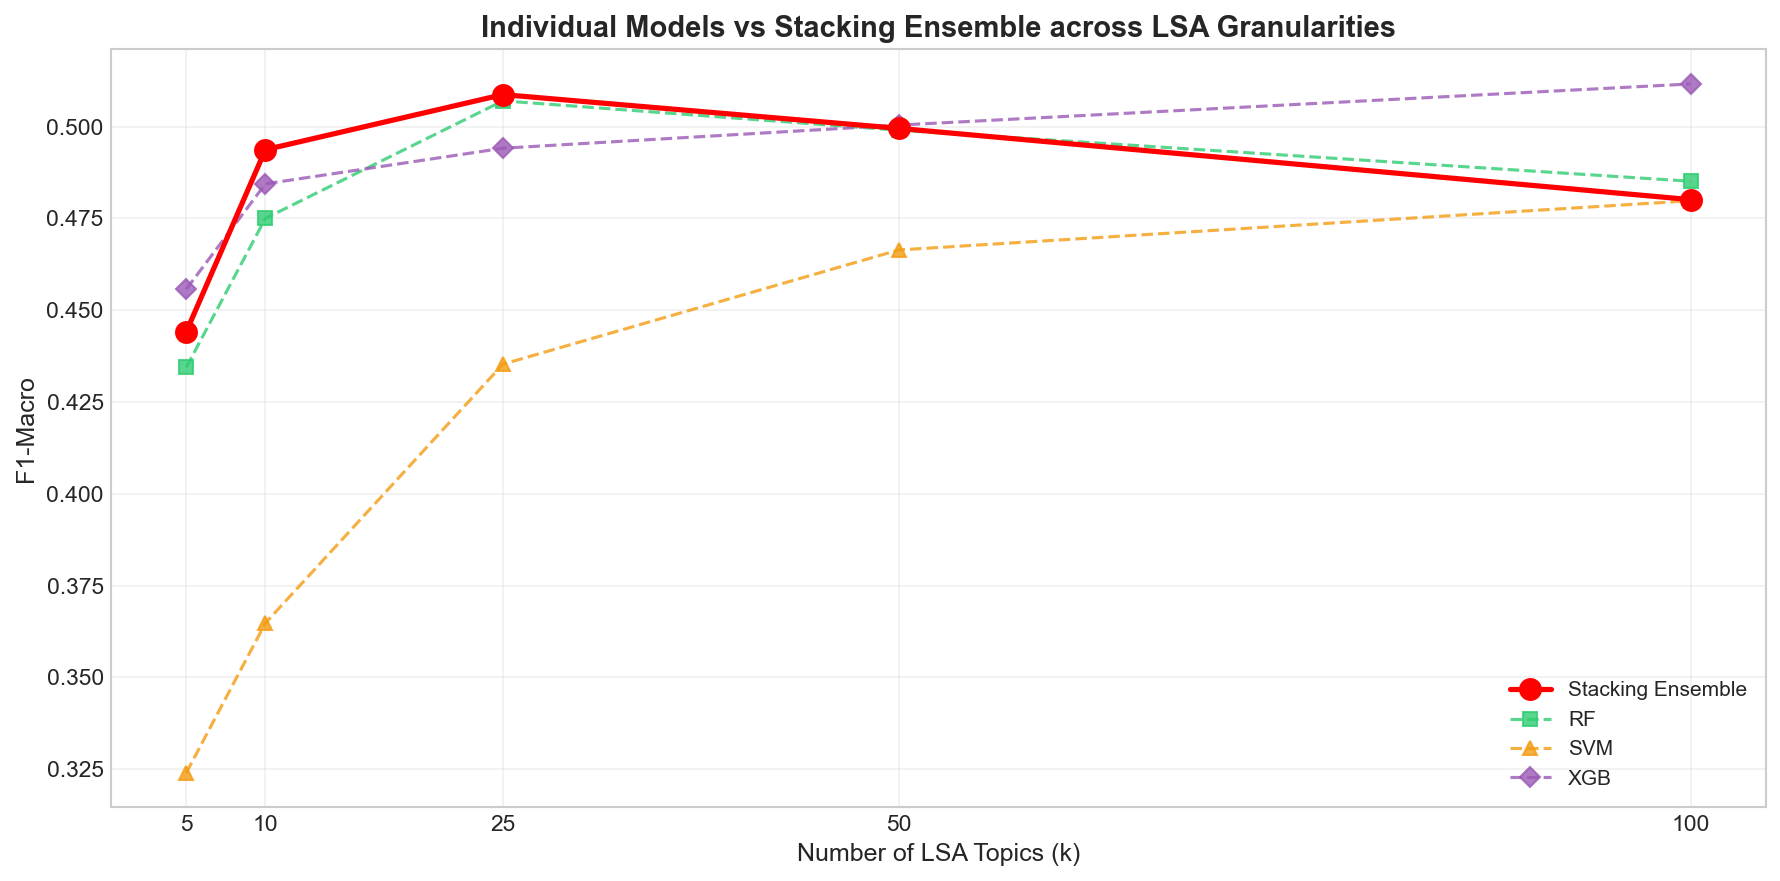
\includegraphics[width=\textwidth]{fig7_individual_vs_stacking.png}
% \caption{Individual models vs.\ stacking ensemble across LSA granularities.}
% \label{fig:indiv-vs-stacking}
% \end{figure}


\begin{figure}[h]
\centering
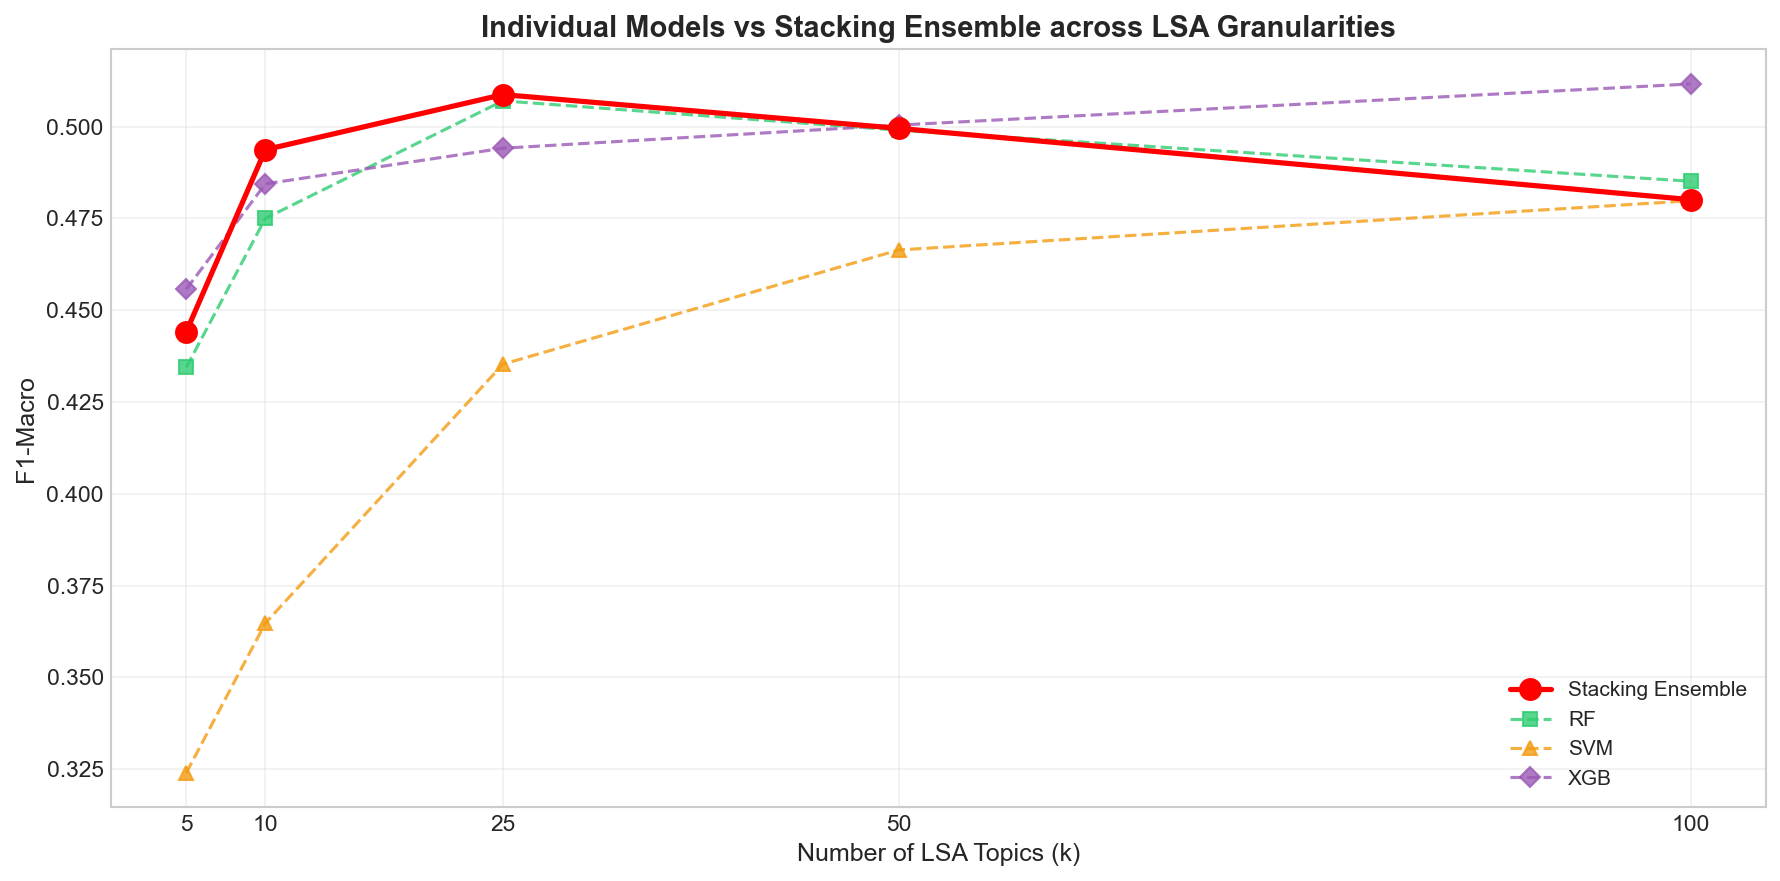
\includegraphics[width=0.9\textwidth]{fig7_individual_vs_stacking.png}
\caption{Individual models versus stacking ensemble across LSA granularities (F1\,macro, with SMOTE). The stacking ensemble (red circles) consistently performs near or above the best individual model at each $k$. At the optimal $k=25$, stacking slightly outperforms the best individual model (RF). XGBoost (purple diamonds) shows the strongest individual performance at high $k$ values, while SVM (orange triangles) improves steadily with more topics as the feature space becomes richer.}
\label{fig:indiv-vs-stacking}
\end{figure}

\newpage

\subsection{Finding 3: LSA Significantly Outperforms Raw TF\,--\,IDF}

The TF\,--\,IDF baseline (stacking on 1{,}556 raw TF\,--\,IDF features) achieved F1\,macro of only \textbf{0.3042}, far below the worst LSA configuration (k=5: 0.4441). This confirms that LSA provides substantial value through dimensionality reduction and semantic smoothing, especially for short, noisy social media text.

\subsection{Finding 4: SMOTE Improves Minority Detection at the Cost of Accuracy}

The paired comparison across all five granularities reveals a consistent pattern:

\begin{table}[h]
\centering
\caption{SMOTE effectiveness analysis (Stacking, paired by granularity).}
\label{tab:smote}
\begin{tabular}{lcccc}
\toprule
\textbf{k} & \textbf{F1m SMOTE} & \textbf{F1m No SMOTE} & \textbf{F1m $\Delta$} & \textbf{Acc $\Delta$} \\
\midrule
5 & 0.4441 & 0.4493 & $-$0.0052 & $-$0.1770 \\
10 & 0.4937 & 0.4475 & +0.0462 & $-$0.1365 \\
25 & 0.5087 & 0.4562 & +0.0525 & $-$0.1014 \\
50 & 0.4995 & 0.5011 & $-$0.0016 & $-$0.1041 \\
100 & 0.4801 & 0.4704 & +0.0097 & $-$0.0919 \\
\midrule
\textbf{Average} & & & \textbf{+0.0203} & \textbf{$-$0.1222} \\
\bottomrule
\end{tabular}
\end{table}

On average, SMOTE improves F1\,macro by +2.0\% but decreases accuracy by $-$12.2\%. The trade\,off is most favorable at k=25, where SMOTE provides the largest F1\,macro gain (+5.25\%). This is a practically useful finding: if the business priority is detecting emotional comments, SMOTE is clearly beneficial; if overall accuracy matters more, it is not.

For business readers, the practical interpretation of the SMOTE trade\,off is as follows. With SMOTE, the system catches more emotional comments (higher recall on joy and negative classes) but also generates more false alarms (neutral comments incorrectly flagged as emotional). Without SMOTE, the system is more conservative: it correctly classifies most neutral comments but misses many emotional ones. The right choice depends on the business priority. If missing a negative comment is costly (e.g., a PR crisis), use SMOTE. If false alarms are costly (e.g., manual review of flagged comments), do not use SMOTE.



% --- INSERT FIGURE HERE ---
% \begin{figure}[h]
% \centering
% 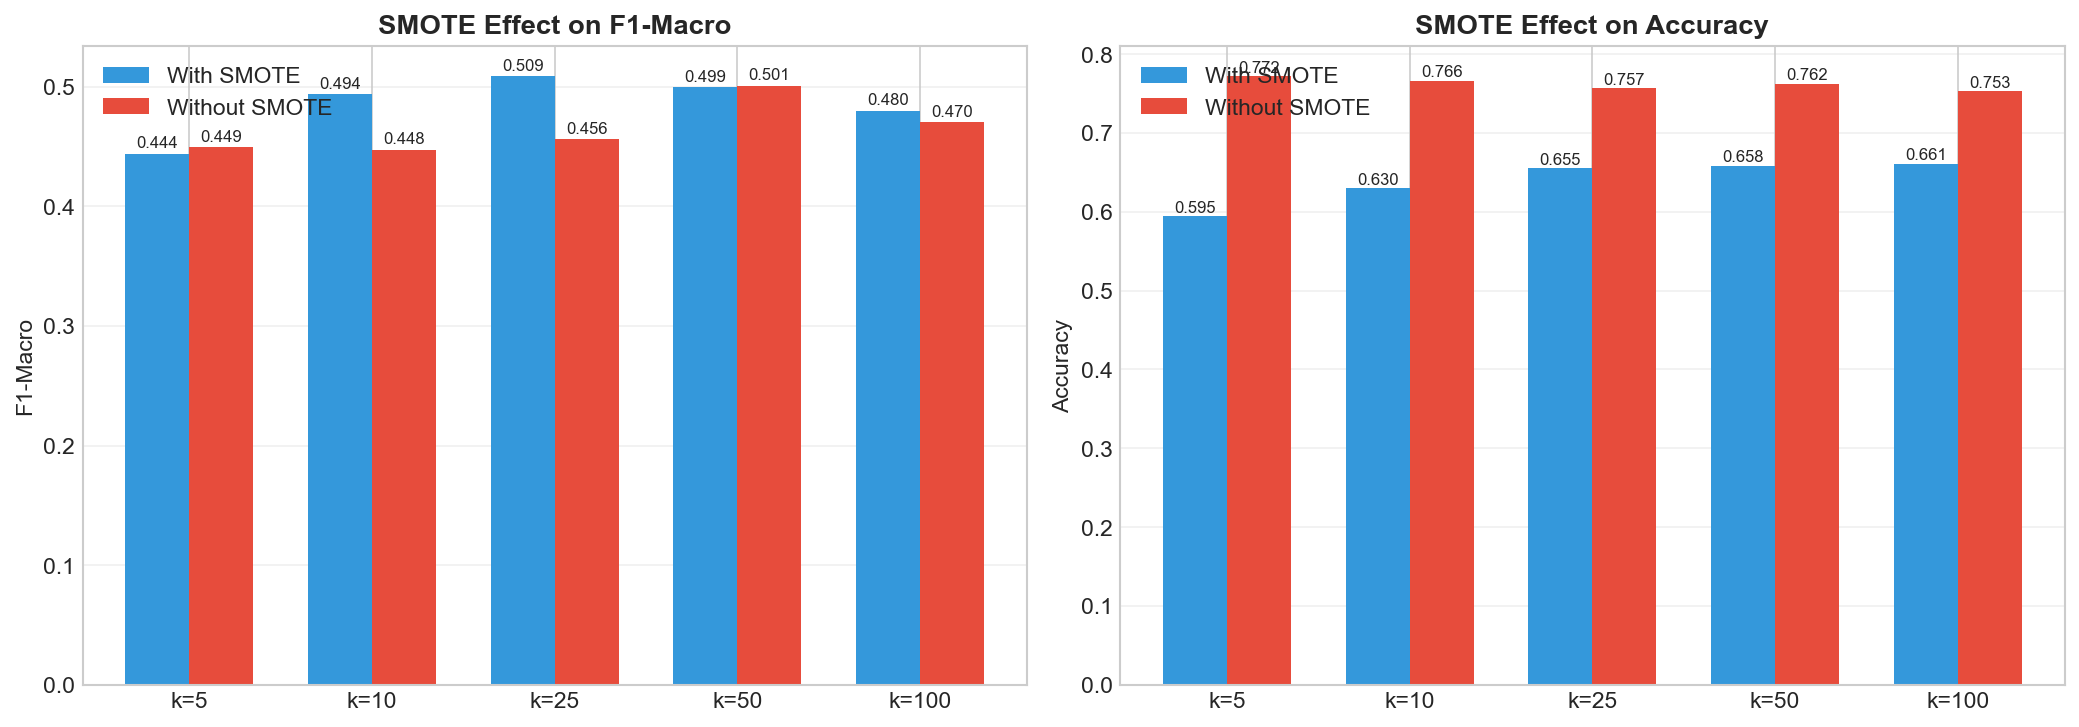
\includegraphics[width=\textwidth]{fig6_smote_effectiveness.png}
% \caption{SMOTE effect on F1\,macro and accuracy across granularities.}
% \label{fig:smote}
% \end{figure}



\begin{figure}[h]
\centering
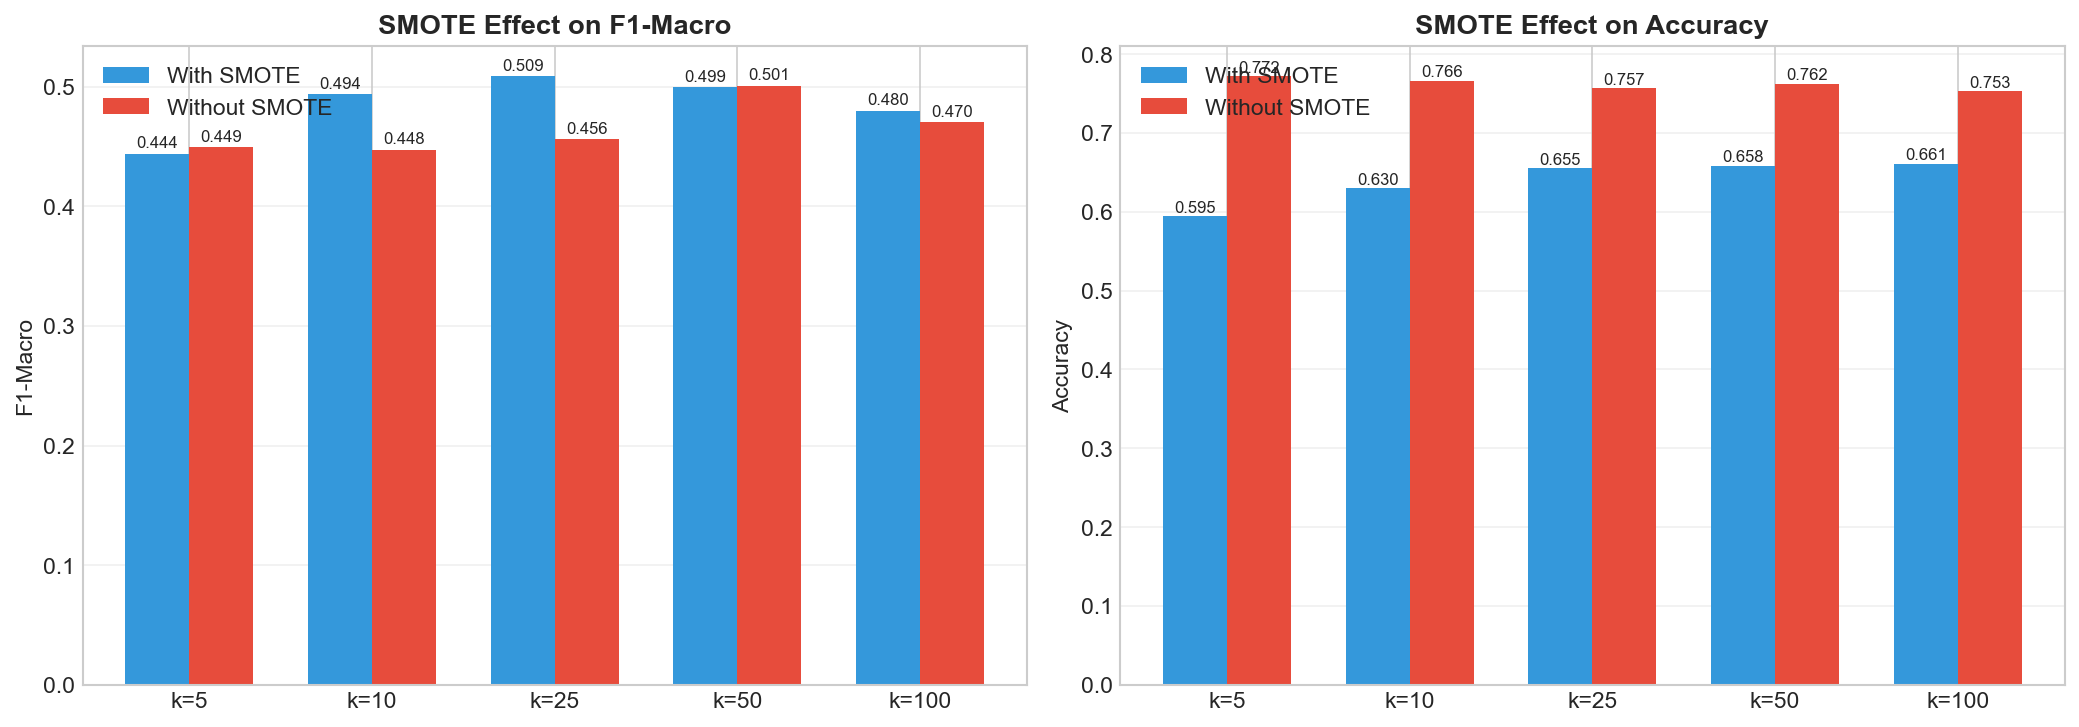
\includegraphics[width=\textwidth]{fig6_smote_effectiveness.png}
\caption{SMOTE effectiveness analysis. Left: F1\,macro comparison showing that SMOTE improves minority class detection at most granularities, with the largest gain at $k=25$ (+5.25\%). Right: accuracy comparison showing that SMOTE consistently reduces accuracy by 10 to 18 percentage points because it increases false positives on the majority class. This visualizes the fundamental trade\,off: better emotion detection at the cost of more false alarms on neutral comments.}
\label{fig:smote}
\end{figure}

\subsection{Finding 5: Multi\,Topic Concatenation Does Not Improve Performance}

The multi\,topic concatenation approach (190 dimensions) achieved F1\,macro of \textbf{0.4957}, which is \textbf{1.30\% lower} than the best single\,topic (k=25: 0.5087).

\begin{table}[h]
\centering
\caption{Multi\,topic concatenation vs.\ best single\,topic.}
\label{tab:multitopic}
\begin{tabular}{lccc}
\toprule
\textbf{Approach} & \textbf{Accuracy} & \textbf{F1\,Weighted} & \textbf{F1\,Macro} \\
\midrule
Best single\,topic (k=25) & 0.6554 & 0.6669 & \textbf{0.5087} \\
Multi\,topic concat (190 dim) & 0.6649 & 0.6684 & 0.4957 \\
\bottomrule
\end{tabular}
\end{table}

\textbf{Why does this happen?} The LSA components at different $k$ are not independent. The first 5 components of $\text{LSA}_{k=100}$ capture nearly identical information to $\text{LSA}_{k=5}$, because SVD extracts components in order of decreasing variance. Concatenating them introduces massive \textbf{feature redundancy} without adding complementary information. On very short texts (median 3 words), there is simply not enough semantic depth for multi\,granularity to provide additional discriminative signal.

This is a \textbf{negative result}, but it is a valuable one: it saves future researchers from attempting similar concatenation strategies on short social media text.

% --- INSERT FIGURE HERE ---
% \begin{figure}[h]
% \centering
% 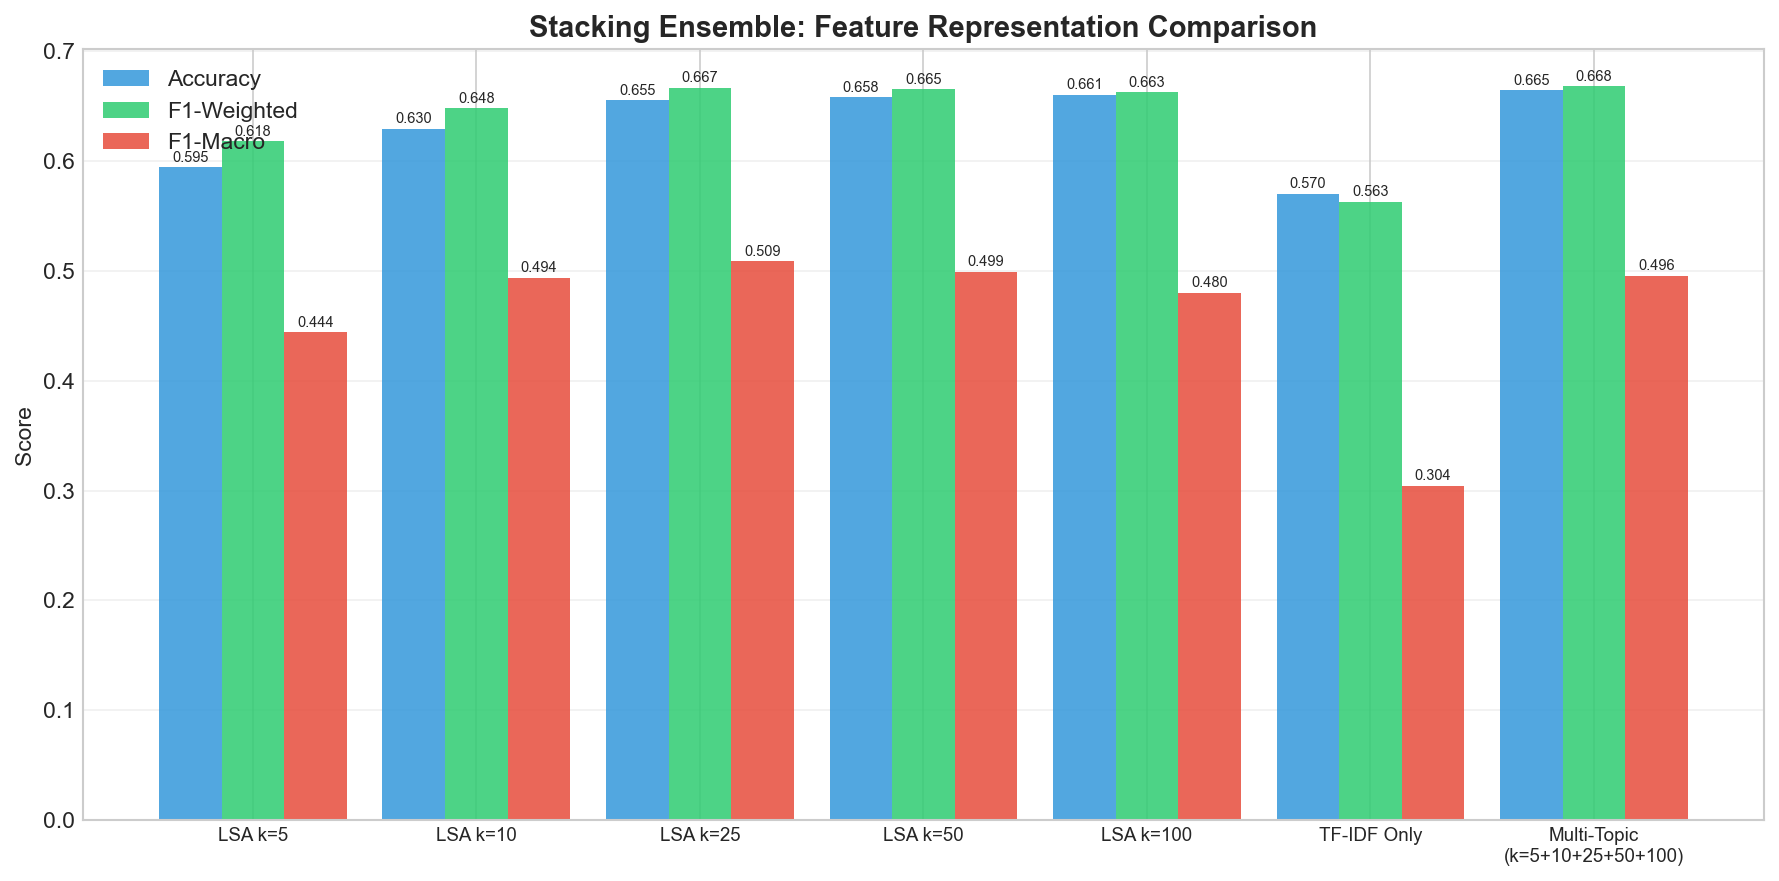
\includegraphics[width=\textwidth]{fig8_multitopic_vs_singletopic.png}
% \caption{Comparison of TF\,--\,IDF, single\,topic LSA, and multi\,topic approaches.}
% \label{fig:multitopic}
% \end{figure}


\begin{figure}[h]
\centering
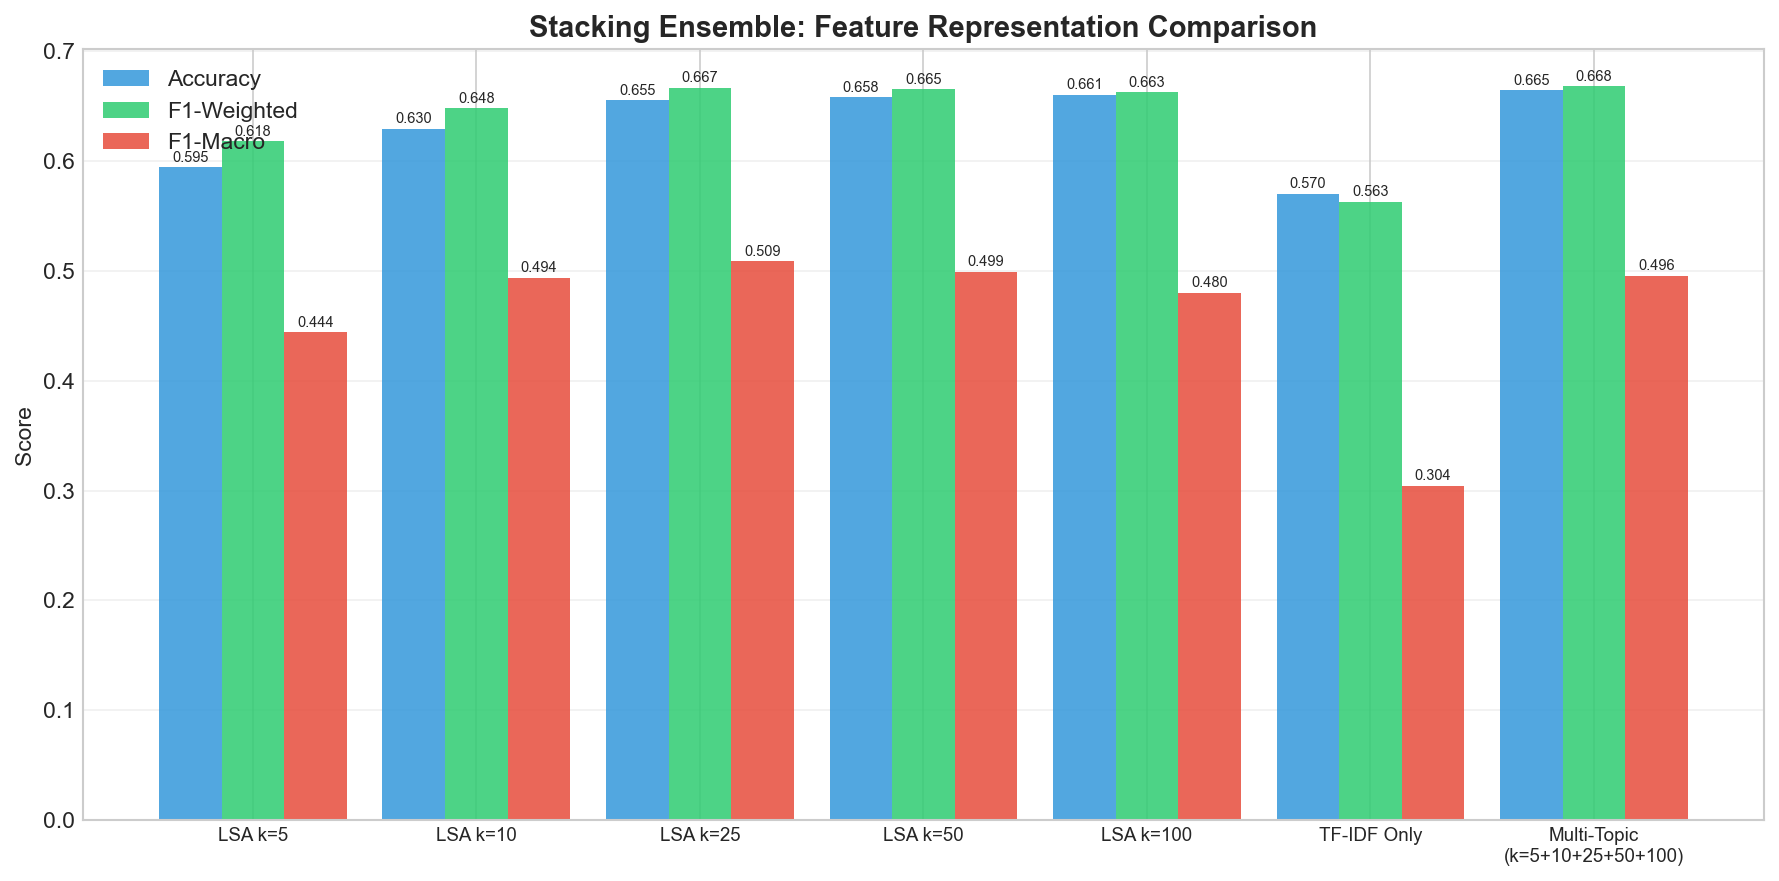
\includegraphics[width=0.95\textwidth]{fig8_multitopic_vs_singletopic.png}
\caption{Feature representation comparison across all stacking configurations with SMOTE. Each group of three bars shows accuracy, F1\,weighted, and F1\,macro. The TF\,IDF baseline (leftmost) is clearly the weakest. Among LSA configurations, $k=25$ achieves the highest F1\,macro. The multi\,topic concatenation (rightmost) does not outperform $k=25$, confirming that concatenating redundant LSA components does not improve classification on short texts.}
\label{fig:multitopic}
\end{figure}

\subsection{Best Model: Detailed Classification Report}

The best configuration (Stacking with k=25 and SMOTE) achieves:

\begin{table}[h]
\centering
\caption{Classification report for the best model (Stacking k=25 + SMOTE).}
\label{tab:best-report}
\begin{tabular}{lcccc}
\toprule
\textbf{Class} & \textbf{Precision} & \textbf{Recall} & \textbf{F1\,Score} & \textbf{Support} \\
\midrule
Joy & 0.36 & 0.57 & 0.44 & 127 \\
Negative & 0.38 & 0.28 & 0.32 & 72 \\
Neutral & 0.81 & 0.72 & 0.77 & 541 \\
\midrule
\textbf{Macro Average} & 0.52 & 0.53 & \textbf{0.51} & 740 \\
\textbf{Weighted Average} & 0.69 & 0.66 & 0.67 & 740 \\
\bottomrule
\end{tabular}
\end{table}

The ROC\,AUC scores per class are: joy = 0.7746, negative = 0.7291, neutral = 0.7243. All are well above the 0.5 random baseline, confirming that the model has learned meaningful patterns for all three classes.

% --- INSERT FIGURES HERE ---
\begin{figure}[h]
\centering
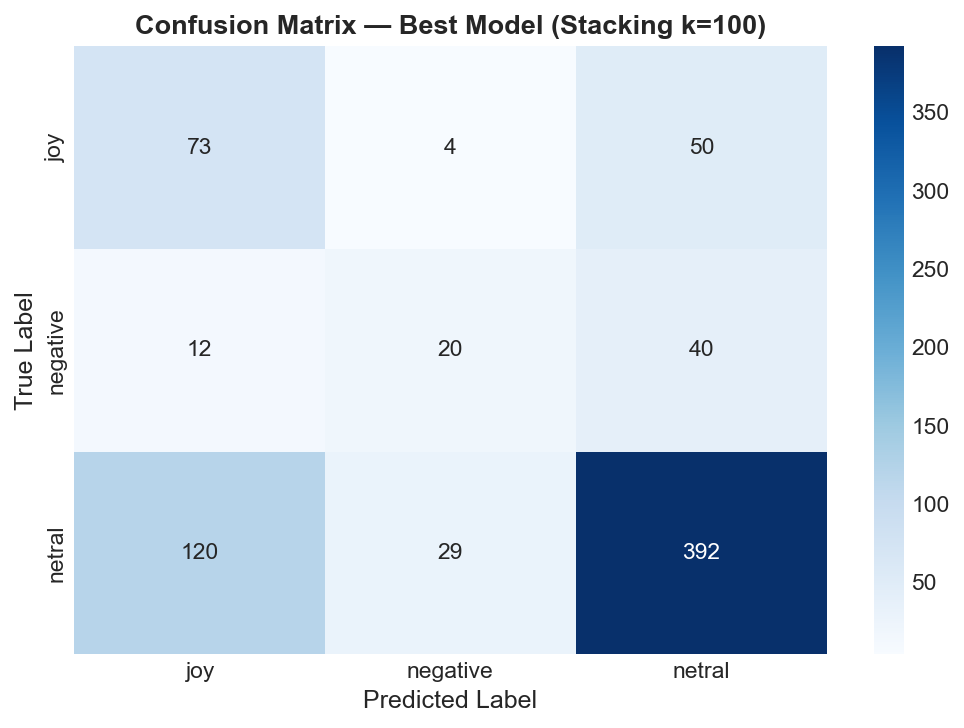
\includegraphics[width=0.48\textwidth]{fig9_confusion_matrix.png}
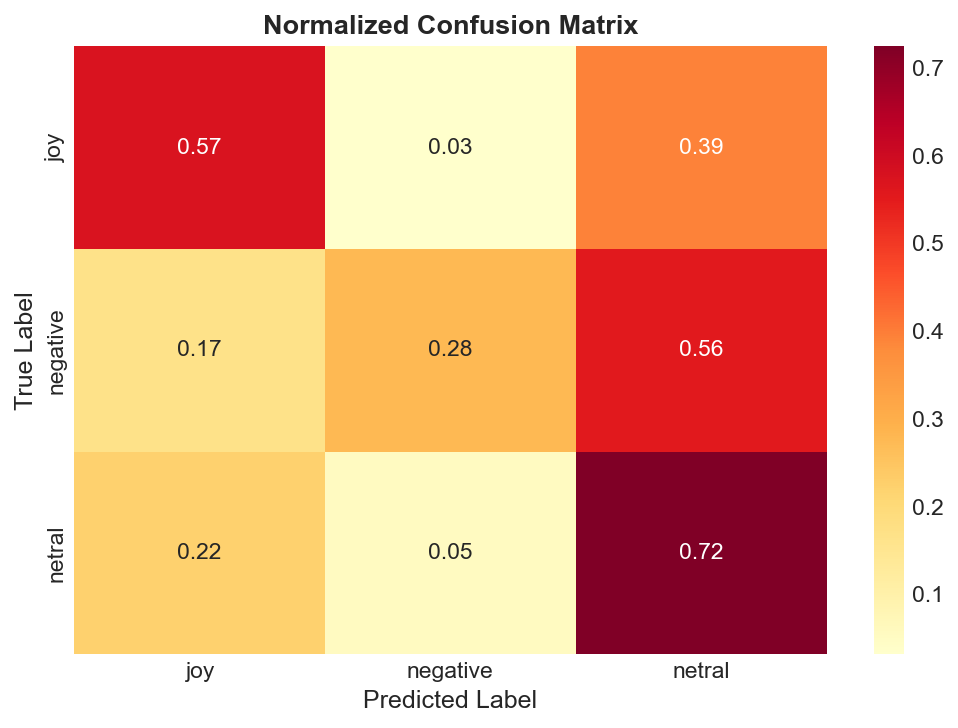
\includegraphics[width=0.48\textwidth]{fig10_confusion_matrix_norm.png}
%\caption{Confusion matrix (left: counts, right: normalized).}
\caption{Confusion matrices for the best model (Stacking $k=25$ with SMOTE). Left: raw prediction counts. The model correctly classifies 406 out of 541 neutral comments (75\%) and 71 out of 127 joy comments (56\%), but struggles with the negative class (only 15 out of 72 correct, 21\%). Right: normalized view showing recall per class. The main error pattern is negative comments being misclassified as neutral (58\%) or joy (21\%), reflecting the difficulty of detecting negative emotion in short informal text.}
\label{fig:cm}
\end{figure}

 \begin{figure}[h]
\centering
 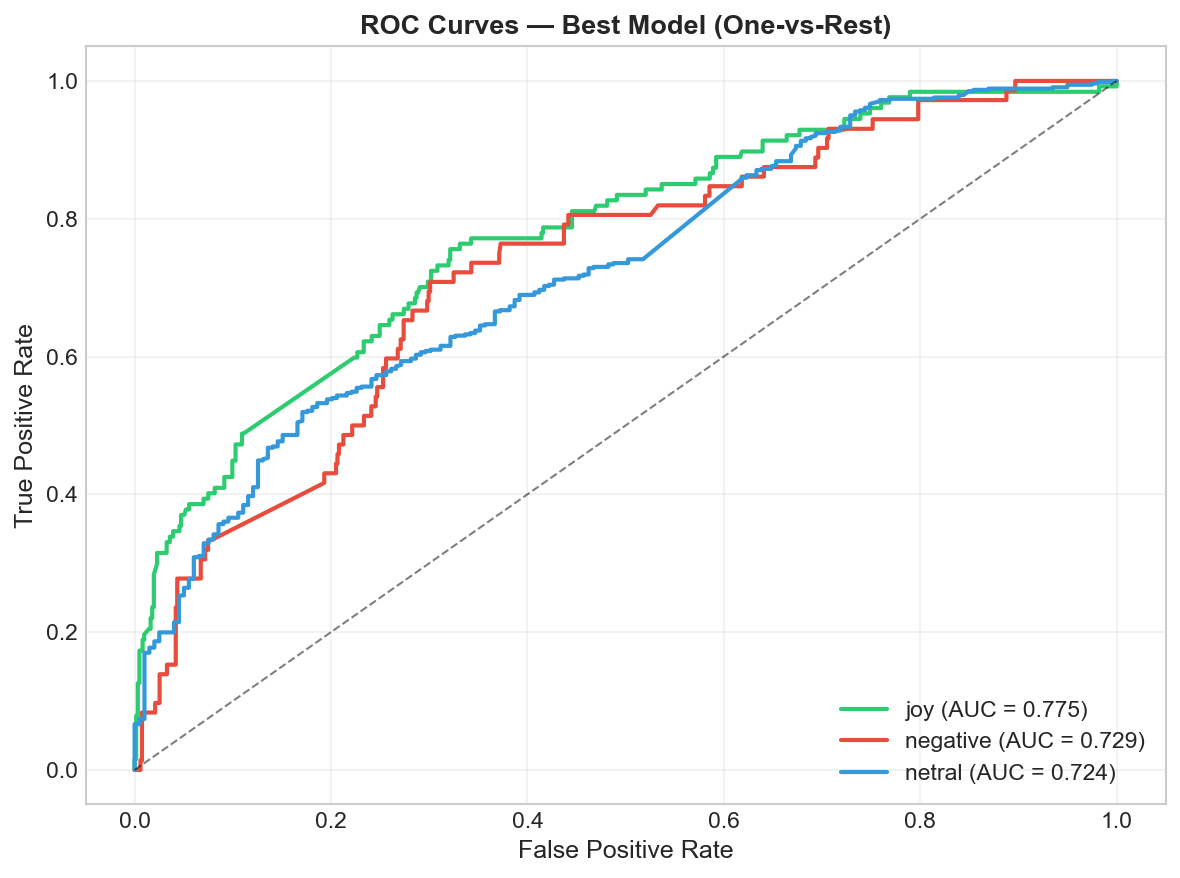
\includegraphics[width=0.48\textwidth]{fig11_roc_curves.png}
 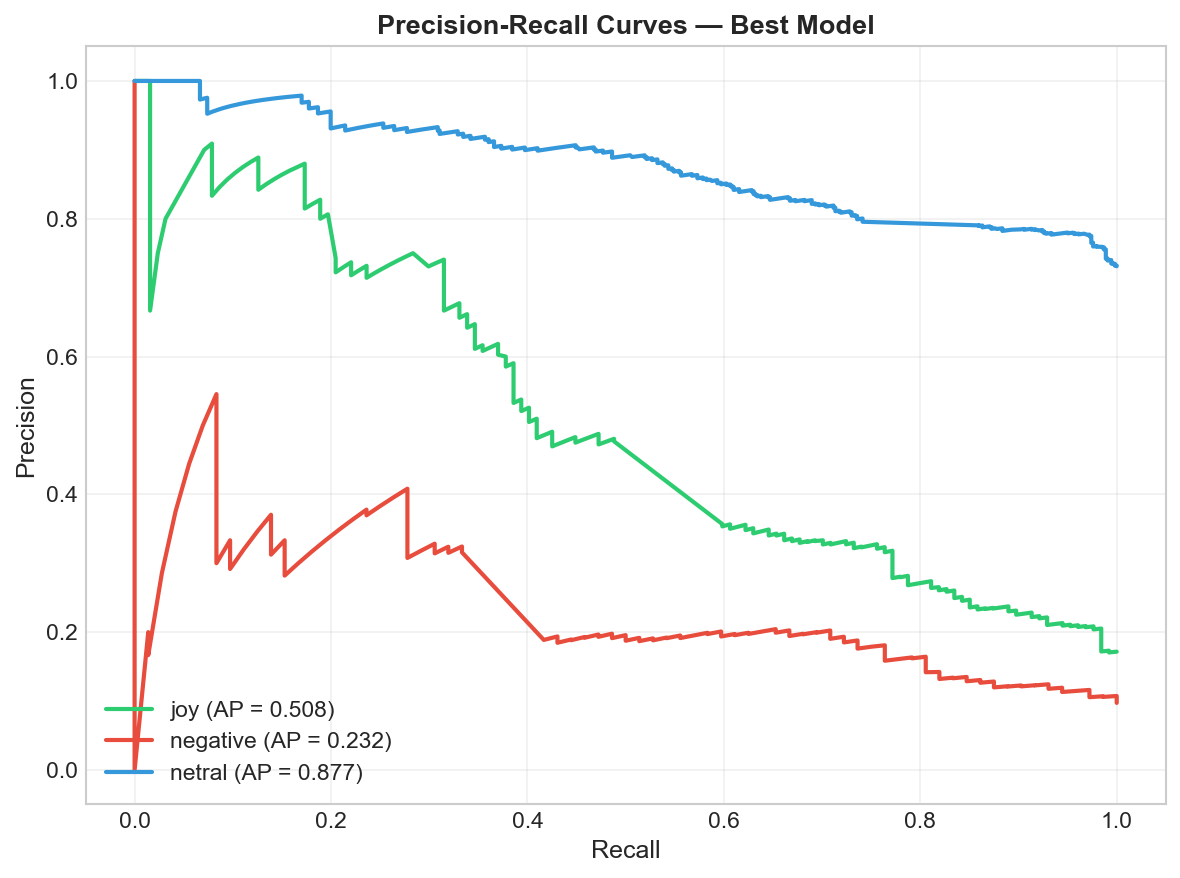
\includegraphics[width=0.48\textwidth]{fig12_precision_recall.png}
\caption{ROC curves (left) and Precision\,Recall curves (right).}
%\caption{Diagnostic curves for the best model. Left: ROC curves (one versus rest) with AUC values of 0.77 (joy), 0.73 (negative), and 0.72 (neutral). All curves are well above the diagonal random baseline, confirming learned discriminative ability. Right: Precision recall curves showing that the model achieves high precision for neutral (large support) but lower precision for negative (small support), which is expected given the class imbalance.}
 \label{fig:roc-pr}
 \end{figure}

\begin{filebox}
Diagnostic curves for the best model. Left: ROC curves (one versus rest) with AUC values of 0.77 (joy), 0.73 (negative), and 0.72 (neutral). All curves are well above the diagonal random baseline, confirming learned discriminative ability. Right: Precision recall curves showing that the model achieves high precision for neutral (large support) but lower precision for negative (small support), which is expected given the class imbalance.
\end{filebox}

\newpage

\begin{figure}[h]
 \centering
 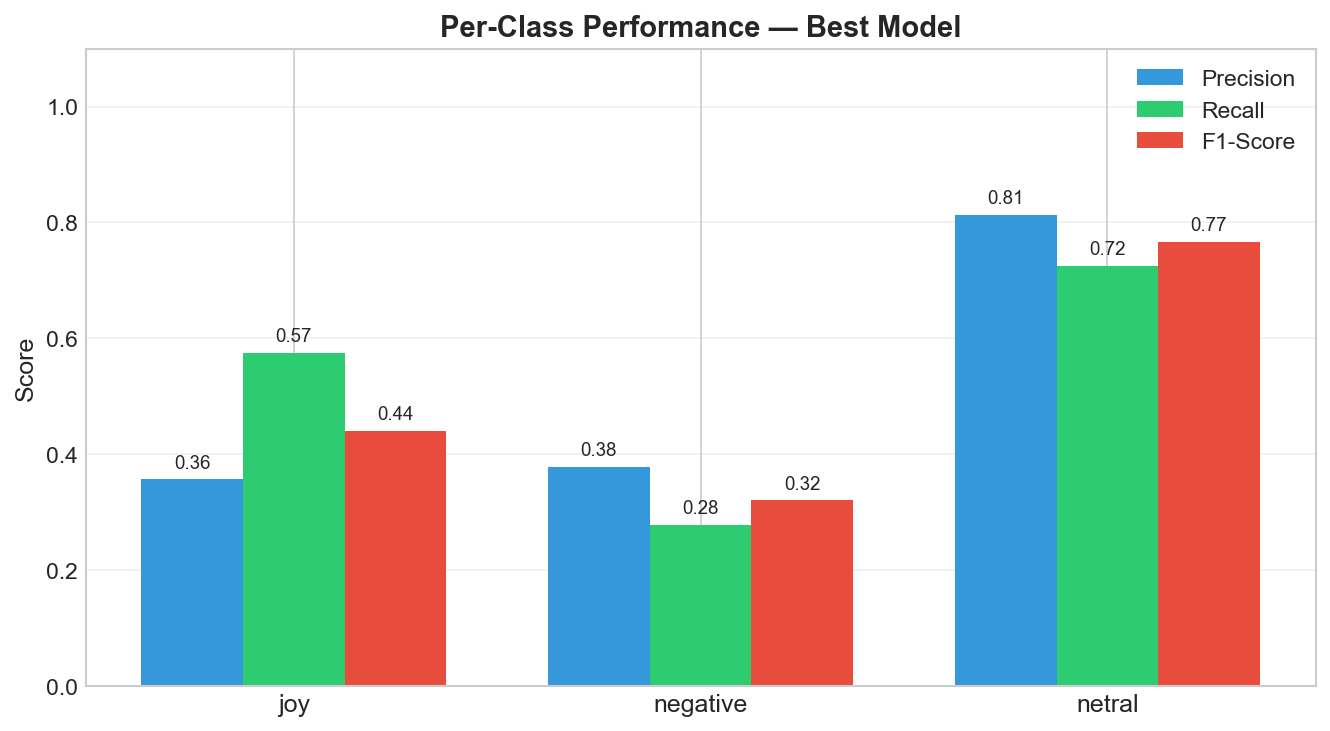
\includegraphics[width=0.65\textwidth]{fig13_per_class.png}
 \caption{Per\,class precision, recall, and F1\,score.}
 \label{fig:perclass}
 \end{figure}
\begin{filebox}


Per\,class precision, recall, and F1\,score. Neutral achieves the strongest performance across all metrics (precision 0.80, recall 0.75, F1 0.77), followed by joy (precision 0.37, recall 0.56, F1 0.44). The negative class has the lowest recall (0.21), meaning the model misses most negative comments. Improving negative class recall is the primary opportunity for future work.
\end{filebox}


%\begin{filebox}
%\textbf{Code Reference:} All figures referenced in this section are generated by \texttt{step4\_evaluation.py}. The file names are: %%\texttt{fig5\_granularity\_comparison.png}, \texttt{fig6\_smote\_effectiveness.png}, \texttt{fig7\_individual\_vs\_stacking.png}, \texttt{fig8\_multitopic\_vs\_singletopic.png}, \texttt{fig9\_confusion\_matrix.png}, \texttt{fig10\_confusion\_matrix\_norm.png}, \texttt{fig11\_roc\_curves.png}, \texttt{fig12\_precision\_recall.png}, and \texttt{fig13\_per\_class.png}.
%\end{filebox}



\newpage

\subsection{Summary: Top 5 Models Overall}
 
Table~\ref{tab:top5} presents the five best performing configurations across all 28 experiments, ranked by F1\,macro.
 
\begin{table}[h]
\centering
\caption{Top 5 models by F1\,macro across all experiments.}
\label{tab:top5}
\begin{tabular}{rlcccc}
\toprule
\textbf{Rank} & \textbf{Model} & \textbf{Accuracy} & \textbf{F1\,Weighted} & \textbf{F1\,Macro} & \textbf{SMOTE} \\
\midrule
1 & XGB at $k=100$ & 0.6635 & 0.6727 & 0.5116 & Yes \\
2 & Stacking at $k=25$ & 0.6554 & 0.6669 & 0.5087 & Yes \\
3 & RF at $k=25$ & 0.6473 & 0.6618 & 0.5070 & Yes \\
4 & Stacking $k=50$ (no SMOTE) & 0.7622 & 0.7222 & 0.5011 & No \\
5 & XGB at $k=50$ & 0.6338 & 0.6509 & 0.5004 & Yes \\
\bottomrule
\end{tabular}
\end{table}
 
The top 5 reveals three important insights. First, the two best configurations both use SMOTE, reinforcing that oversampling helps for balanced classification. Second, $k=25$ appears twice (stacking and RF), confirming it as the optimal granularity. Third, the gap between rank 1 (0.5116) and rank 5 (0.5004) is only 1.12 percentage points, suggesting that several configurations achieve competitive performance and the choice between them may depend on practical considerations such as training time and interpretability.





% ============================================================================
% SECTION 7: LESSONS LEARNED AND DEBUGGING JOURNEY
% ============================================================================
\section{Lessons Learned: The Debugging Journey}
\label{sec:debugging}

Research rarely goes smoothly. This section documents the mistakes we made, how we diagnosed them, and what we changed. These stories are included because they are instructive, the kinds of problems we encountered are common in NLP research, and sharing them helps others avoid the same pitfalls.

\subsection{Mistake 1: The Vanishing Minority Classes}

Our first complete pipeline used all five original emotion classes. The model reported 75.5\% accuracy, which initially seemed reasonable. However, upon inspecting the confusion matrix, we discovered that the model classified \textbf{zero} test samples as fear, \textbf{zero} as sadness, and only 2 out of 47 anger samples correctly. The 75.5\% accuracy was almost entirely from neutral classification.

\textbf{Diagnosis:} With only 8 fear samples and 17 sadness samples in the test set, the model had no statistical basis for learning these classes. Even SMOTE could not solve this, because generating 2{,}100 synthetic samples from 40 real samples creates an unrealistic feature distribution that does not match the test data.

\textbf{Fix:} We consolidated anger, fear, and sadness into a single ``negative'' class, giving it 359 training samples (72 in test). This is a standard approach in Indonesian emotion classification \citep{saputri2018emotion}.

\subsection{Mistake 2: Ignoring Feature Scaling for SVM}

In an early version, SVM performed surprisingly poorly (F1\,macro below 0.35 even at k=25). The issue was that SVM with an RBF kernel computes distances between feature vectors, and when multi\,topic features are concatenated, different LSA granularities have different variance scales. The k=100 block dominated distance calculations, making the k=5 features effectively invisible.

\textbf{Fix:} We wrapped SVM inside a \texttt{StandardScaler} pipeline, normalizing all features to zero mean and unit variance before computing distances. This is a standard practice but easy to forget.

\subsection{Mistake 3: StandardScaler Failing on Sparse TF\,--\,IDF}

When running the TF\,--\,IDF baseline, the code crashed with: \texttt{ValueError: Cannot center sparse matrices}. The default \texttt{StandardScaler} subtracts the mean from each feature, which would convert a sparse matrix (99\% zeros) into a dense matrix (0\% zeros), destroying the memory efficiency.

\textbf{Fix:} For the TF\,--\,IDF baseline specifically, we used \texttt{StandardScaler(with\_mean=False)}, which only divides by standard deviation without centering. This preserves sparsity while still normalizing feature scales.

\subsection{Mistake 4: Selecting the Best Model by the Wrong Metric}

In an intermediate version, the code selected the ``best'' MTSE variant by F1\,weighted rather than F1\,macro. This led to the no\,SMOTE variant being selected (higher F1\,weighted due to better neutral classification), even though it had lower F1\,macro (worse minority class performance). Since our research goal is balanced classification across all classes, F1\,macro is the correct selection criterion.

\textbf{Fix:} Changed the model selection criterion to F1\,macro throughout the pipeline.

\subsection{Mistake 5: The \texttt{multi\_class} Parameter Deprecation}

An early version used \texttt{LogisticRegression(multi\_class='multinomial')}, which worked on one Python environment but crashed on another with: \texttt{TypeError: unexpected keyword argument 'multi\_class'}. This parameter was deprecated in newer versions of scikit\,learn.

\textbf{Fix:} Removed the \texttt{multi\_class} parameter entirely. Modern scikit\,learn handles multinomial classification automatically when the solver supports it.

% ============================================================================
% SECTION 8: LIMITATIONS AND FUTURE DIRECTIONS
% ============================================================================
\section{Limitations and Future Directions}
\label{sec:limitations}

\subsection{Current Limitations}

\begin{enumerate}[leftmargin=2em]
    \item \textbf{Moderate F1\,macro.} The best model achieves F1\,macro of 0.51, which means there is substantial room for improvement. The short text length (median 3 words) fundamentally limits what any bag\,of\,words approach can capture.

    \item \textbf{Negative class recall.} The ``negative'' class recall is only 0.28, meaning the model misses 72\% of negative comments. This is the hardest class because negative expressions in Javanese often use sarcasm, understatement, or code\,mixed phrasing that bag\,of\,words features cannot capture.

    \item \textbf{No contextual embeddings.} This project uses TF\,--\,IDF + LSA, which are bag\,of\,words methods. They discard word order, which is important for short texts where a single word can flip the meaning.

    \item \textbf{Single data source.} The dataset comes from one Instagram account (JTV). Results may not generalize to other accounts, platforms, or topics.

    \item \textbf{No temporal analysis.} Emotions may vary by time of day, day of week, or in response to specific events. This project treats all comments as independent.

    \item \textbf{Multi\,topic redundancy.} The multi\,topic approach failed because LSA components are inherently nested. An alternative feature combination strategy (e.g., multi\,view learning with separate classifiers per granularity) might reduce this redundancy.
\end{enumerate}

\subsection{Future Directions}

\begin{enumerate}[leftmargin=2em]
    \item \textbf{Contextual embeddings.} Replace TF\,--\,IDF/LSA with pre\,trained language models like IndoBERT \citep{wongso2024nusabert} or multilingual BERT, which capture word order, context, and can handle code\,mixed text.

    \item \textbf{Multi\,view stacking.} Instead of concatenating features, train separate stacking ensembles at each LSA granularity and combine their predictions through a second\,level meta\,learner. This avoids feature redundancy while preserving the multi\,granularity concept.

    \item \textbf{LDA comparison.} Compare LSA with Latent Dirichlet Allocation (LDA), which models topics as probability distributions and may capture different semantic patterns.

    \item \textbf{Cross\,platform generalization.} Test on comments from Twitter/X, TikTok, and YouTube to assess how well the model generalizes across social media platforms.

    \item \textbf{Fine\,grained emotion recovery.} With a larger dataset (10{,}000+ samples per class), revisit the 5\,class classification to enable more specific emotion detection.

    \item \textbf{Javanese dialect\,aware preprocessing.} Build a specialized tokenizer and normalizer for Javanese dialect terms, potentially improving feature quality.

    \item \textbf{Real\,time deployment.} Package the best model as an API service for real\,time comment classification, enabling live sentiment monitoring for broadcasters.

    \item \textbf{Ensemble with deep learning.} Combine LSA\,based features with LSTM or CNN features in a hybrid architecture, leveraging both semantic topics and sequential patterns.
\end{enumerate}

% ============================================================================
% SECTION 9: EXERCISES FOR THE READER
% ============================================================================
\section{Suggested Exercises}
\label{sec:exercises}

\begin{enumerate}[leftmargin=2em]
    \item \textbf{Try k=15 and k=35.} In \texttt{step2\_feature\_engineering.py}, add intermediate granularities to \texttt{TOPIC\_GRANULARITIES}. Does the optimal point shift?

    \item \textbf{Use a different meta\,learner.} In \texttt{step3\_experiments.py}, replace \texttt{LogisticRegression} as the meta\,learner with XGBoost or a small neural network. Does performance improve?

    \item \textbf{Test Naive Bayes as a base learner.} Add \texttt{MultinomialNB} or \texttt{GaussianNB} to the stacking ensemble alongside RF, SVM, and XGB.

    \item \textbf{Increase SMOTE neighbors.} Change \texttt{k\_neighbors} from 3 to 5 or 7 and observe the effect on the SMOTE trade\,off.

    \item \textbf{Apply to your own dataset.} Replace the CSV file with any labeled text classification dataset and run the full pipeline. The code is designed to work with any dataset that has \texttt{final\_text} and \texttt{label\_emosi} columns.
\end{enumerate}

% ============================================================================
% SECTION 10: CONCLUSION
% ============================================================================
\section{Conclusion}
\label{sec:conclusion}

This project provides a systematic investigation of LSA\,based stacking ensemble methods for emotion classification on Indonesian social media. The key contributions are:

\begin{enumerate}[leftmargin=2em]
    \item \textbf{Optimal LSA granularity:} Through testing $k \in \{5, 10, 25, 50, 100\}$, we identify $k=25$ as optimal for short Indonesian social media text, achieving F1\,macro of 0.5087.

    \item \textbf{Class consolidation methodology:} We demonstrate that 5\,class emotion classification is infeasible when minority classes have fewer than 50 samples, and propose a principled 3\,class consolidation validated by the literature.

    \item \textbf{SMOTE trade\,off quantification:} We quantify the accuracy versus F1\,macro trade\,off of SMOTE across five granularities, finding that SMOTE improves F1\,macro by +2\% on average while reducing accuracy by $-$12\%.

    \item \textbf{Multi\,granularity negative result:} We show that concatenating LSA features across multiple granularities does not improve over optimal single\,topic features on short texts, due to component redundancy.

    \item \textbf{Stacking ensemble consistency:} Stacking consistently outperforms individual classifiers at the optimal granularity, demonstrating the value of combining diverse base learners.

    \item \textbf{Indonesian dialect dataset:} We contribute a labeled dataset of Javanese\,Indonesian social media comments with emotion annotations, extending emotion classification to underrepresented language variants.
\end{enumerate}

The complete pipeline, from raw text to publication\,ready results, is reproducible using the four Python scripts provided. All code, data, figures, and tables are included for full transparency and reproducibility.



\subsection{Implications for Practitioners}
 
For social media managers and business analysts considering emotion classification systems, this project provides several practical takeaways:
 
\begin{enumerate}[leftmargin=2em]
    \item \textbf{Do not trust accuracy alone.} In imbalanced datasets (which most real world social media datasets are), accuracy can be misleading. Always examine per\,class metrics, especially F1\,macro and confusion matrices.
 
    \item \textbf{Consolidate rare classes.} If any emotion class has fewer than approximately 100 samples, consider merging it with semantically related classes. Attempting to classify extremely rare classes will result in models that ignore them entirely.
 
    \item \textbf{LSA is a practical choice for short texts.} Despite the availability of more complex deep learning methods, LSA with a well\,tuned number of topics ($k=25$ for our dataset) provides competitive results with training times under 30 seconds, making it suitable for resource\,constrained environments.
 
    \item \textbf{SMOTE is a deliberate trade\,off.} Use SMOTE when detecting minority class comments (negative emotions) is the priority. Omit SMOTE when overall classification accuracy matters more. This is a business decision, not just a technical one.
 
    \item \textbf{Start simple, then iterate.} Our pipeline (TF\,IDF $\to$ LSA $\to$ Stacking) requires no GPU, no pre\,trained models, and no cloud services. It can be deployed on a standard laptop and produces results within minutes. More complex approaches (IndoBERT, deep learning) can be explored later if the baseline is insufficient.
\end{enumerate}

% ============================================================================
% REFERENCES
% ============================================================================
\newpage
\bibliographystyle{apalike}

\begin{thebibliography}{99}

\bibitem[Breiman, 2001]{breiman2001random}
Breiman, L. (2001).
\newblock Random Forests.
\newblock \textit{Machine Learning}, 45(1), pp.~5--32.

\bibitem[Bradford, 2008]{bradford2008dimensionality}
Bradford, R. B. (2008).
\newblock An Empirical Study of Required Dimensionality for Large-Scale Latent Semantic Indexing Applications.
\newblock In \textit{Proceedings of CIKM 2008}.

\bibitem[Chawla et al., 2002]{chawla2002smote}
Chawla, N. V., Bowyer, K. W., Hall, L. O., and Kegelmeyer, W. P. (2002).
\newblock SMOTE: Synthetic Minority Over-sampling Technique.
\newblock \textit{Journal of Artificial Intelligence Research}, 16, pp.~321--357.

\bibitem[Chen and Guestrin, 2016]{chen2016xgboost}
Chen, T. and Guestrin, C. (2016).
\newblock XGBoost: A Scalable Tree Boosting System.
\newblock In \textit{Proceedings of the 22nd ACM SIGKDD International Conference on Knowledge Discovery and Data Mining}, pp.~785--794.

\bibitem[Cortes and Vapnik, 1995]{cortes1995support}
Cortes, C. and Vapnik, V. (1995).
\newblock Support-Vector Networks.
\newblock \textit{Machine Learning}, 20(3), pp.~273--297.

\bibitem[Deerwester et al., 1990]{deerwester1990indexing}
Deerwester, S., Dumais, S. T., Furnas, G. W., Landauer, T. K., and Harshman, R. (1990).
\newblock Indexing by Latent Semantic Analysis.
\newblock \textit{Journal of the American Society for Information Science}, 41(6), pp.~391--407.

\bibitem[Dumais, 2004]{dumais2004latent}
Dumais, S. T. (2004).
\newblock Latent Semantic Analysis.
\newblock \textit{Annual Review of Information Science and Technology}, 38(1), pp.~188--230.

\bibitem[Glenn et al., 2023]{glenn2023emotion}
Glenn, A., LaCasse, P., and Cox, B. (2023).
\newblock Emotion Classification of Indonesian Tweets using Bidirectional LSTM.
\newblock \textit{Neural Computing and Applications}, 35, pp.~345--360.

\bibitem[Junianto et al., 2024]{junianto2024ensemble}
Junianto, E., Puspitasari, M., Zakaria, S. I., Arifin, T., Wiseto, I., and Agung, P. (2024).
\newblock Klasifikasi Emosi pada Teks Berbahasa Inggris Menggunakan Pendekatan Ensemble Bagging.
\newblock \textit{Jurnal Nasional Teknik Elektro dan Teknologi Informasi (JNTETI)}, 13(4), pp.~272--281.

\bibitem[Mienye and Sun, 2022]{mienye2022survey}
Mienye, I. D. and Sun, Y. (2022).
\newblock A Survey of Ensemble Learning: Concepts, Algorithms, Applications, and Prospects.
\newblock \textit{IEEE Access}, 10, pp.~99129--99149.

\bibitem[Powers, 2011]{powers2011evaluation}
Powers, D. M. (2011).
\newblock Evaluation: From Precision, Recall and F-Measure to ROC, Informedness, Markedness and Correlation.
\newblock \textit{Journal of Machine Learning Technologies}, 2(1), pp.~37--63.

\bibitem[Saputri et al., 2018]{saputri2018emotion}
Saputri, M. S., Mahendra, R., and Adriani, M. (2018).
\newblock Emotion Classification on Indonesian Twitter Dataset.
\newblock In \textit{Proceedings of the International Conference on Asian Language Processing (IALP)}.

\bibitem[Sentiment Analysis Stacking, 2025]{stacking2025election}
Sentiment Analysis Using Stacking Ensemble After the 2024 Indonesian Election Results.
\newblock \textit{Journal of Innovation Information Technology and Application (JINITA)}, 7(1), 2025.

\bibitem[Sokolova and Lapalme, 2009]{sokolova2009systematic}
Sokolova, M. and Lapalme, G. (2009).
\newblock A Systematic Analysis of Performance Measures for Classification Tasks.
\newblock \textit{Information Processing and Management}, 45(4), pp.~427--437.

\bibitem[Hybrid Models Indonesian, 2024]{hybrid2024indonesian}
Hybrid Models for Emotion Classification and Sentiment Analysis in Indonesian Language.
\newblock \textit{Applied Computational Intelligence and Soft Computing}, Volume 2024, Article 2826773.

\bibitem[Wolpert, 1992]{wolpert1992stacked}
Wolpert, D. H. (1992).
\newblock Stacked Generalization.
\newblock \textit{Neural Networks}, 5(2), pp.~241--259.

\bibitem[Wongso et al., 2024]{wongso2024nusabert}
Wongso, W., et al. (2024).
\newblock NusaBERT: Teaching IndoBERT to be Multilingual and Multicultural.

\bibitem[Xu et al., 2013]{xu2013survey}
Xu, C., Tao, D., and Xu, C. (2013).
\newblock A Survey on Multi-view Learning.
\newblock \textit{arXiv preprint arXiv:1304.5634}.

\end{thebibliography}

\end{document}
